\PassOptionsToPackage{unicode=true}{hyperref} % options for packages loaded elsewhere
\PassOptionsToPackage{hyphens}{url}
%
\documentclass[]{book}
\usepackage{lmodern}
\usepackage{amssymb,amsmath}
\usepackage{ifxetex,ifluatex}
\usepackage{fixltx2e} % provides \textsubscript
\ifnum 0\ifxetex 1\fi\ifluatex 1\fi=0 % if pdftex
  \usepackage[T1]{fontenc}
  \usepackage[utf8]{inputenc}
  \usepackage{textcomp} % provides euro and other symbols
\else % if luatex or xelatex
  \usepackage{unicode-math}
  \defaultfontfeatures{Ligatures=TeX,Scale=MatchLowercase}
\fi
% use upquote if available, for straight quotes in verbatim environments
\IfFileExists{upquote.sty}{\usepackage{upquote}}{}
% use microtype if available
\IfFileExists{microtype.sty}{%
\usepackage[]{microtype}
\UseMicrotypeSet[protrusion]{basicmath} % disable protrusion for tt fonts
}{}
\IfFileExists{parskip.sty}{%
\usepackage{parskip}
}{% else
\setlength{\parindent}{0pt}
\setlength{\parskip}{6pt plus 2pt minus 1pt}
}
\usepackage{hyperref}
\hypersetup{
            pdftitle={Philosophical Ethics},
            pdfauthor={George W. Matthews},
            pdfborder={0 0 0},
            breaklinks=true}
\urlstyle{same}  % don't use monospace font for urls
\usepackage[margin=3cm]{geometry}
\usepackage{longtable,booktabs}
% Fix footnotes in tables (requires footnote package)
\IfFileExists{footnote.sty}{\usepackage{footnote}\makesavenoteenv{longtable}}{}
\usepackage{graphicx,grffile}
\makeatletter
\def\maxwidth{\ifdim\Gin@nat@width>\linewidth\linewidth\else\Gin@nat@width\fi}
\def\maxheight{\ifdim\Gin@nat@height>\textheight\textheight\else\Gin@nat@height\fi}
\makeatother
% Scale images if necessary, so that they will not overflow the page
% margins by default, and it is still possible to overwrite the defaults
% using explicit options in \includegraphics[width, height, ...]{}
\setkeys{Gin}{width=\maxwidth,height=\maxheight,keepaspectratio}
\setlength{\emergencystretch}{3em}  % prevent overfull lines
\providecommand{\tightlist}{%
  \setlength{\itemsep}{0pt}\setlength{\parskip}{0pt}}
\setcounter{secnumdepth}{5}
% Redefines (sub)paragraphs to behave more like sections
\ifx\paragraph\undefined\else
\let\oldparagraph\paragraph
\renewcommand{\paragraph}[1]{\oldparagraph{#1}\mbox{}}
\fi
\ifx\subparagraph\undefined\else
\let\oldsubparagraph\subparagraph
\renewcommand{\subparagraph}[1]{\oldsubparagraph{#1}\mbox{}}
\fi

% set default figure placement to htbp
\makeatletter
\def\fps@figure{htbp}
\makeatother

\usepackage[Bjornstrup]{fncychap}

\usepackage{booktabs}
\usepackage{longtable}
\usepackage[bf,singlelinecheck=off]{caption}

%\setmainfont[UprightFeatures={SmallCapsFont=AlegreyaSC-Regular}]{Alegreya}

\usepackage{framed,color}
\definecolor{shadecolor}{RGB}{248,248,248}

\renewcommand{\textfraction}{0.05}
\renewcommand{\topfraction}{0.8}
\renewcommand{\bottomfraction}{0.8}
\renewcommand{\floatpagefraction}{0.75}

%\renewenvironment{quote}{\begin{VF}}{\end{VF}}
\let\oldhref\href
\renewcommand{\href}[2]{#2\footnote{\url{#1}}}

\ifxetex
  \usepackage{letltxmacro}
  \setlength{\XeTeXLinkMargin}{1pt}
  \LetLtxMacro\SavedIncludeGraphics\includegraphics
  \def\includegraphics#1#{% #1 catches optional stuff (star/opt. arg.)
    \IncludeGraphicsAux{#1}%
  }%
  \newcommand*{\IncludeGraphicsAux}[2]{%
    \XeTeXLinkBox{%
      \SavedIncludeGraphics#1{#2}%
    }%
  }%
\fi%

\makeatletter
\newenvironment{kframe}{%
\medskip{}
\setlength{\fboxsep}{.8em}
 \def\at@end@of@kframe{}%
 \ifinner\ifhmode%
  \def\at@end@of@kframe{\end{minipage}}%
  \begin{minipage}{\columnwidth}%
 \fi\fi%
 \def\FrameCommand##1{\hskip\@totalleftmargin \hskip-\fboxsep
 \colorbox{shadecolor}{##1}\hskip-\fboxsep
     % There is no \\@totalrightmargin, so:
     \hskip-\linewidth \hskip-\@totalleftmargin \hskip\columnwidth}%
 \MakeFramed {\advance\hsize-\width
   \@totalleftmargin\z@ \linewidth\hsize
   \@setminipage}}%
 {\par\unskip\endMakeFramed%
 \at@end@of@kframe}
\makeatother

\makeatletter
\@ifundefined{Shaded}{
}{\renewenvironment{Shaded}{\begin{kframe}}{\end{kframe}}}
\makeatother


\newenvironment{rmdblock}[1]
  {
  \begin{itemize}
  \renewcommand{\labelitemi}{
    \raisebox{-.7\height}[0pt][0pt]{
      {\setkeys{Gin}{width=3em,keepaspectratio}\includegraphics{img/#1}}
    }
  }
  \setlength{\fboxsep}{1em}
  \begin{kframe}
  \item
  }
  {
  \end{kframe}
  \end{itemize}
  }
\newenvironment{rmdnote}
  {\begin{rmdblock}{note}}
  {\end{rmdblock}}
\newenvironment{rmdcaution}
  {\begin{rmdblock}{caution}}
  {\end{rmdblock}}
\newenvironment{rmdimportant}
  {\begin{rmdblock}{important}}
  {\end{rmdblock}}
\newenvironment{rmdtip}
  {\begin{rmdblock}{tip}}
  {\end{rmdblock}}
\newenvironment{rmdwarning}
  {\begin{rmdblock}{warning}}
  {\end{rmdblock}}
\newenvironment{rmdquestion}
  {\begin{rmdblock}{question}}
  {\end{rmdblock}}
\newenvironment{rmdslides}
  {\begin{rmdblock}{slides}}
  {\end{rmdblock}}

\newenvironment{epigraph}%
{
\begin{flushright}
\begin{minipage}{20em}
\begin{flushright}
\itshape
}%
{
\end{flushright}
\end{minipage}
\end{flushright}
\vspace{1em}
}



\newenvironment{argument}{\begin{quote}\normalsize}{\end{quote}}
\usepackage[]{natbib}
\bibliographystyle{plainnat}

\title{Philosophical Ethics}
\providecommand{\subtitle}[1]{}
\subtitle{A Guidebook for Beginners}
\author{\textbf{George W. Matthews}}
\date{last revised: 2019-12-06}

\begin{document}
\maketitle

{
\setcounter{tocdepth}{2}
\tableofcontents
}
\hypertarget{preface}{%
\chapter*{Preface}\label{preface}}


\textbf{\emph{This book}} is an introduction to philosophical ethics intended for use in introductory college or high school level courses. It has grown out of lecture notes I shared with the first students who took my online Ethics course at the Pennsylvania College of Technology almost 20 years ago. Since then it has seen more development in a variety of forms -- starting out as a pdf document, and then evolving into a static set of WordPress pages and finally now as a book written in bookdown and hosted at GitHub. This text represents my attempt to scratch a few itches. The first is my wanting a presentation of the major philosophical approaches to ethics that I can actually agree with and that is integrated into my overall teaching method. I tend to teach philosophy to beginners and so there is a fair amount of discussion of the tools used by philosophers and of the ways in which their approach differs from that of their colleagues in other disciplines.

\textbf{\emph{There are}} of course many good quality ethics textbooks out there, and yet none has exactly matched my way of wanting to present the material. Teaching ethics over the years has been a process of active exploration and constant revision of my approach as I have come to a more nuanced and richer appreciation of what ethical thinking and theorizing is all about, as well as some ideas about how I think the main strands of argument relate to each other. Yes this is a partisan effort, but it's all subject to revision and refinement based on, I hope at least, the better argument. That's what I am trying to get across here.

\textbf{\emph{The second itch}} I am trying to scratch here has to do with initiatives in open education, and I'd like this text to contribute in its own small way to the much larger and more influential open source movement and philosophy of which I consider it a part. Knowledge is only ours to share. Yes of course writers, developers and publishers do hard work that deserves compensation. But intellectual property, it seems to me, is a false idol that deserves to be smashed. So here is my effort to chip away at it -- knowledge should free us and and not sink us into both literal and figurative debt.

\textbf{\emph{In addition}} the decision to convert this text into a \href{https://github.com/gwmatthews/ethics}{GitHub repository} should be considered as an invitation for others to participate in its future development. Anyone can fork the repository where it resides and use it as a template for their own book project; offer suggestions for revisions, or contribute in other ways as well. Please use the ``issues'' section of the repository for making any major suggestions.

\hypertarget{dedication}{%
\section*{Dedication}\label{dedication}}


\begin{epigraph}
Receive correctly this monk's word-stream, neither frozen nor trickling
away, neither transparent nor muddy. When you wring it dry, take
advantage of the opportunity; when you enter the bustle, perceive with
your whole eye. Thorough understanding and the changing world fulfill
each other totally without obstacle. The moon accompanies the current,
the wind bends the grass\ldots{}Find your seat, wear your robe, and go
forward and see for yourself.

---Hongzhi, \emph{Cultivating the Empty Field}
\end{epigraph}

\begin{center}
\includegraphics[width=0.5\linewidth]{img/hongzhi} \end{center}

\hypertarget{acknowledgements}{%
\section*{Acknowledgements}\label{acknowledgements}}


\textbf{\emph{The writing}} and publication of this book would not have been possible without the work of numerous people who make and share their amazing work in the open source software community. It is based in particular on the work of \href{https://github.com/yihui}{Yi Hui} and the other developers of \href{https://github.com/rstudio/bookdown}{bookdown} and \href{https://rstudio.com/products/rstudio/}{Rstudio} and related software. While it has been a bit of a steep learning curve figuring out how to use Rstudio and bookdown to write and style a book, it has been a lot of fun too! The end product, hopefully, speaks for itself and demonstrates that these tools are not just for people with highly technical backgrounds, but can be used by anyone with some computer skills and a bit of patience to create functional, cross-platform and pretty good looking web based books.

Icons are by Paul Davey aka \href{http://mattahan.deviantart.com}{Mattahan}. All rights reserved.

\begin{center}
\includegraphics[width=0.43in]{img/tux} \end{center}

\hypertarget{license-cc-by-sa-4.0}{%
\subsection*{License CC BY-SA 4.0}\label{license-cc-by-sa-4.0}}


\textbf{\emph{This book}} is released under a creative commons \href{https://creativecommons.org/licenses/by-sa/4.0/}{CC BY-SA 4.0} license. This means that this book can be reused, remixed, retained, revised and redistributed (including commercially) as long as appropriate credit is given to the authors. If you remix, or modify the original version of this open textbook, you must redistribute all versions of this open textbook under the same license.

\hypertarget{how-to-use-this-book}{%
\section*{How to use this book}\label{how-to-use-this-book}}


\hypertarget{read-it}{%
\subsection*{Read it}\label{read-it}}


This should be self-explanatory, but be sure not to miss the icons on the top of the screen which enable you to:

\begin{itemize}
\tightlist
\item
  Open up and close the sidebar with the table of contents in it.
\item
  Search within the text for a keyword.
\item
  Change the color scheme or font to make it easier to read.
\item
  Offer editorial suggestions on GitHub (see below for how this works).
\item
  Download a pdf version of the text for offline reading or printing.
\item
  Find out keyboard short cuts for navigation.
\end{itemize}

Also note the arrows on the side of the screen (or down at the bottom if you are reading on a small screen) that bring you to the next or previous pages.

\hypertarget{comment-on-it}{%
\subsection*{Comment on it}\label{comment-on-it}}


If you are a current student in one of my Ethics classes you'll have to do some commenting. When I used WordPress to host this text that was a built in feature. Here I am relying on a third party commenting add-on to the online version of the book. There are many ways to do this, with Disqus being one of the most popular. I chose to use a system called \href{https://www.remarkbox.com/}{Remarkbox} for the following reasons:

\begin{enumerate}
\def\labelenumi{\arabic{enumi}.}
\tightlist
\item
  They do NOT track users.
\item
  And so there is NO targeted advertising that you will be exposed to just by responding to a page in an online textbook, in fact there is no advertising at all.
\item
  It is an open source project that was created by someone as an alternative to other commenting systems like Disqus that DO track users and inundate them with ads.
\end{enumerate}

To use this system you will have to enter a valid email address and then click on a link in the email this system sends you and then whatever comments you make will be stored on the Remarkbox servers. You can see exactly what they store by reading their \href{https://www.remarkbox.com/privacy-policy.html}{privacy policy}.

When you first use the system you will get a random bunch of characters as your user name. If you are a student in my classes please change this to the format Your-first-nameLast-initial: So John Smith would be JohnS and I am GeorgeM. That's just so I can keep track of who is commenting how much for grading purposes.

\begin{rmdimportant}
\textbf{How to comment}

\begin{enumerate}
\def\labelenumi{\arabic{enumi}.}
\tightlist
\item
  Type your comment in the box at the bottom of the page -- you can
  format it using
  \href{https://www.markdownguide.org/basic-syntax/}{markdown} or just
  write in plain text.
\item
  Enter a valid email address in the box below.
\item
  Click the ``save message'' button.
\item
  Go to your email inbox, open the message from Remarkbox and click on
  the link there.
\item
  You will be redirected back to the page you commented on and will now
  be logged in.
\item
  If this is your first comment, you can change your user name by
  clicking on the letter in a colored circle next to the ``watch''
  button -- that will open up ``user settings'' where you can change
  your user name to something like SheenaE (if you happen to be Sheena
  Easton).
\item
  You can also log out, and either follow or unfollow any comment
  threads you like by clicking on the appropriate buttons.
\item
  If you get stuck with your settings open, you can use the back button
  or your browser or refresh the page to return to the comments. (Seems
  like a bug to me, honestly, but this is software in active
  development.)
\end{enumerate}
\end{rmdimportant}

Others are also welcome to comment on the text. Please be respectful though or you might get banned.

\hypertarget{contribute-to-it}{%
\subsection*{Contribute to it}\label{contribute-to-it}}


If you find a mistake, don't think it's clear in some part, have an issue with any part of it, want something more added, etc. I encourage you to contribute. You can do this in a couple of ways.

\begin{itemize}
\tightlist
\item
  Leave a comment and we can discuss possible changes.
\item
  Click on the ``edit'' button on the top menu bar -- this will take you to the GitHub repository where the source material lives. There you can either open up an ``issue'' and we can discuss it there, or you can ``fork'' the repository make whatever edits you want and then offer them in the form of a ``pull request.'' All of this assumes that you:

  \begin{itemize}
  \tightlist
  \item
    Know what ``git'' even is.\footnote{If you don't, it is a version control system that enables collaboration and it mostly intended for software development, but it can be used for working together on any kind of project that involves electronic files, from novels to operating systems. If you want to learn more, check out \href{https://happygitwithr.com/}{Happy Git and GitHub for the useR} or \href{https://www.atlassian.com/git/tutorials/learn-git-with-bitbucket-cloud}{Learn git with Bitbucket Cloud}. I love reading documentation, don't you?}
  \item
    Have an account at \href{https://github.com/}{GitHub} -- which is free. And \href{https://pages.github.com/}{GitHub pages} is a great way to get yourself a free website too!
  \end{itemize}
\item
  Send me an email if you know me in the real world.
\end{itemize}

\hypertarget{part-some-preliminaries}{%
\part*{Some Preliminaries}\label{part-some-preliminaries}}


\hypertarget{the-examined-life}{%
\chapter{The Examined Life}\label{the-examined-life}}

\begin{center}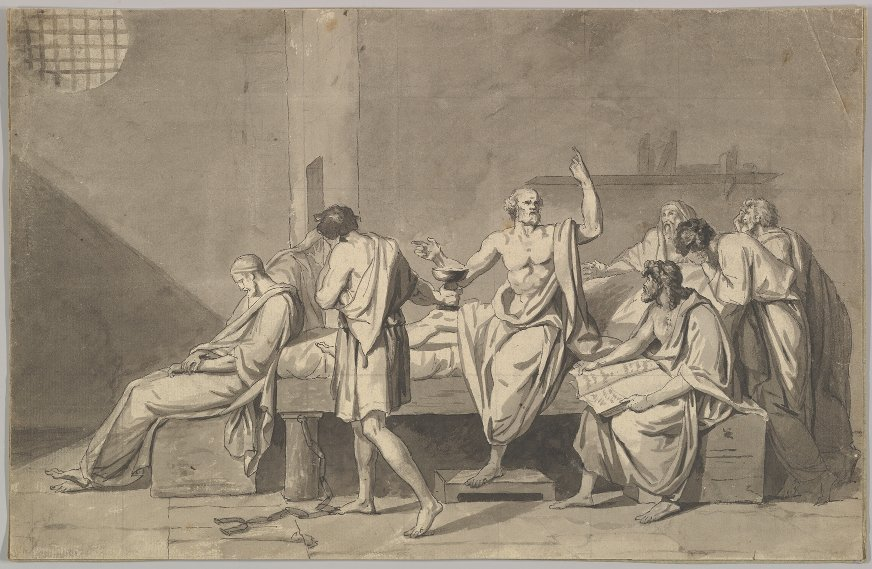
\includegraphics[width=0.6\linewidth]{img/david-socrates} \end{center}

\begin{epigraph}
The unexamined life is not worth living.

---Socrates
\end{epigraph}

\textbf{\emph{Human beings}} are endowed with a unique capacity, the ability to reflect on what we believe and do. Unlike other animals, we are capable of taking a distance from the evidence of our senses and asking ourselves, ``Should I trust what I see or not?'' Likewise in the realm of desire and action: we can examine our own desires, intentions and plans and ask ourselves, ``Should I act on these or not?'' In both cases we are capable of stepping back from the immediate demands of our situation and seeking orientation from another source -- we seek \emph{reasons} to believe or doubt what we see and \emph{reasons} to follow or resist our urges. This reflective capacity is the source of our strength since it has enabled us to both understand and manipulate the world around us like no other creature on the planet. But it also puts us in the uniquely awkward position of having to justify ourselves to our own worst critics, ourselves.

\textbf{\emph{Shakespeare's tragic figure}} of Hamlet sums this up quite well when he on the one hand proclaims,

\begin{quote}
What a piece of work is a man! how noble in reason! how infinite in faculties! in form and moving how express and admirable! in action how like an angel! in apprehension how like a god! the beauty of the world, the paragon of animals! And yet to me what is this quintessence of dust?
\end{quote}

\textbf{\emph{The capacity}} to reflect is the source of both our godlike ``apprehension'' and the difficulties we inevitably encounter in figuring out what we should do. Even though, thankfully, most of us do not experience the tension between these two aspects of our ability to reflect on ourselves and our circumstances quite as dramatically as Hamlet did, all of us face this essentially human predicament. As we will be seeing in this text, philosophical ethics is another, much less bloody, way of exploring this predicament. To set the stage for what we will be up to here I want to first say a bit more about our unique reflective capacity and our ability to pay attention to reasons. Then I'll turn to a more detailed account of what is distinctive about philosophy in general and philosophical ethics in particular.

\hypertarget{what-do-i-know}{%
\section{What do I know?}\label{what-do-i-know}}

\textbf{\emph{To start out}} I don't want to exaggerate too much our differences from the other organisms with which we share the planet, since we do have quite a bit with in common with them. We may be, as Aristotle's definition of human beings has it, ``rational animals,'' but we are still animals, and like all other animals with nervous systems we can do two things. We can perceive what is happening around us and we can respond to it in real time. Animal nervous systems are the product of hundreds of millions of years of evolution, and extremely useful for helping animals survive and flourish in a complex and constantly changing environment. What is distinctive about the human nervous system is the degree to which the constant stream of information coming into it through our senses is integrated and organized. It is integrated in an experience which is, as far as we can tell, more fully conscious than in other creatures. And it is organized more explicitly, as is especially evident in our ability to use language.

\textbf{\emph{And likewise}} with the equally constant stream of information produced by our nervous systems, controlling our bodily and verbal responses and the way these both in turn feed back on our thought processes. That these are capable of being integrated and organized in ways that are unique to human is clearly demonstrated in the astonishing variety and complexity of human cultural and social forms. Of course animals out-perform humans in a variety of specialized tasks, but human achievements in the worlds of culture and society are seemingly capable of infinite variation and complexity ranging from Simone Biles to the internet, from the modern corporation to Tuvan throat singing.

\textbf{\emph{Above all}} it is our capacity for language use that makes possible the integration and organizational flexibility of the human mind. As just one example of how this works, our ability to use and understand language enables us to explicitly categorize and classify what we experience -- things are not just there in our surroundings as objects we happen to come across. Instead we both consciously and unconsciously organize the things we encounter into groups based on concepts such as: edible or inedible, animate or inanimate, threatening or safe, members of our social group or not members of our group, male or female, cause or effect, and so on. Now although there is clear evidence that many animals do this to a limited extent as well -- dogs, for example distinguish between their owners and strangers, vervet monkeys make different alarm calls for different predators -- for us, these acts of categorizing and classifying can be endlessly expanded and modified and also made fully explicit to our own awareness. We can endlessly expand our categories to include anything and everything conceivable - ``80's hair bands,'' ``things not good for eating in bed,'' ``mops,'' and ``former presidents,'' just to give a quick random sample.

\textbf{\emph{Not only do we}} thus have an infinitely variable way of looking at the world and organizing our experience according to concepts and categories, but we can see and understand how we are doing so by reflecting on it and talking about it. We can make it explicit how our experience of things is organized and maybe even do it in a different way. We can add new categories or modify how we use them as we notice new similarities or subtle distinctions among things. We may also revise and refine our categories as accumulated personal and shared experience reveals to us their strengths and weaknesses -- whether they ``carve nature at its joints'' or not. This ability to look at things in new ways as a result of collectively accumulated experience is rooted in the fact that we use language to do so and language is both infinitely extensible and essentially shared with other humans. Most importantly for the story I am telling here, we can ask ourselves about the implications of the way we look at the world, and we can wonder about whether we \emph{really} have good reasons for looking at things as we do.

\textbf{\emph{This is a point}} that it is hard to overemphasize but also easy to miss since we take it so much for granted. By asking ourselves about the reasons we have for believing that some aspect or other of our experience is true we are asking ourselves not only about the way things are, but about the way things \emph{should} be; not just what we happen to believe about things based on their appearance to us, but about what we \emph{should} believe about them because it reflects their true reality. And by asking ourselves such questions we are asking what philosophers call normative questions, questions that have to do with values, with concepts like right, wrong, good, bad, true, false, beautiful and ugly.

\hypertarget{what-should-i-do}{%
\section{What should I do?}\label{what-should-i-do}}

\textbf{\emph{Thus far}} I have been emphasizing the role of reflection and the seeking of reasons in our attempts to understand the world in which we live. But this of course is an incomplete picture, since we are not just disembodied minds looking at and trying to figure out the world. We are embodied, social beings who feel and act on needs and impulses, experience emotions, form and try to realize intentions, coordinate or compete with others, and seek or shun each others' company. This practical side of human life is, just as we have seen for our experiential selves, equally capable of being made explicit and becoming an object of our reflective capacities. We don't have to simply act on whatever urges happen to come to our attention, we can stop and think about what to do instead. Hence we find ourselves presented with choices -- should I follow my immediate urges, or should I refrain from doing so in order to realize other goals?

\textbf{\emph{Once again}}, just as in the case of belief, our reflective capacity introduces a normative dimension to human life as we come to ask ourselves questions about our own needs, desires and decisions. We may wonder what we should do in some particular situation, perhaps when our feelings are telling us one thing and our experience is reminding us of the bad results the last time we acted on similar impulses. And this generalizes as well -- as we come to reflect on our motivations as such, on which of our goals are more worth pursuing in the long run, on the nature of human motivation and goals in general, and on what might truly be the best way to live our lives. And thus philosophical ethics is born as a product of reflection on our own decision making as potentially thoughtful social animals.

\hypertarget{a-difficult-case}{%
\subsection*{A difficult case}\label{a-difficult-case}}


\begin{rmdquestion}
Imagine that you are standing next to a railway track and notice a
runaway trolley coming down the tracks. There are five children further
down the track who are too far away to hear you. There is also a switch
in front of you, that would divert the trolley to the other track.
Unfortunately there is also a single worker on the other track, who is
himself to far away to hear you.

\emph{Would you throw the switch and cause the worker to most likely die
in order to prevent the runaway trolley from hitting the children?}
\end{rmdquestion}

\textbf{\emph{This classic case}} of an ethical dilemma has been extensively studied by philosophers and psychologists. One significant result of these studies is that a large majority of people say that if they were in that situation they \emph{would} throw the switch. That is they are following a common moral intuition that might be expressed by the rule: all else being equal do whatever saves the most lives. Consider, however, the following variation on this case.

\begin{rmdquestion}
Imagine that you are standing on a bridge with a low railing over a
railway track and notice a runaway trolley coming down the tracks. There
are five children further down the track who are too far away to hear
you. There is also a very large person standing next to you, and if you
gave him a slight push he would fall in front of the trolley car causing
it to derail, thus saving the five children.

\emph{Would you push the person off of the bridge in order to prevent
the runaway trolley from hitting the children?}
\end{rmdquestion}

\textbf{\emph{In this case}} a large majority of people say they \emph{would not} push the person off of the bridge even if it would save the five children. Given that the result is the same in either case, the question then becomes why it is that in the first version of this scenario no longer look at it in terms of the intuition that it is better to do what leads to more lives being saved.

\textbf{\emph{Whatever the explanation}} for this discrepancy may be (and there is an entire academic industry that has developed around research into the trolley dilemma) the important point here is that philosophers are interested both in reflecting on cases like this and in studying how it is that we all reflect on similar cases. In the next section we will look briefly at the kinds of questions that dilemmas like this might raise and at what is distinctive about the philosophical approach.

\hypertarget{philosophical-ethics}{%
\section{Philosophical Ethics}\label{philosophical-ethics}}

\textbf{\emph{Philosophical ethics}} is nothing but the deliberate pursuit and clarification of this kind of reflection on our own values, actions and decisions. Even though, as I have been emphasizing, we all have the capacity to reflect on our lives and choices, we do not always spend the time or make the effort to do this carefully and deeply. This is because we are mostly preoccupied with the practical details of our own lives. We are too busy living to take the time to stop and think about the significance of what we are doing. However, at times in the lives of both individuals and societies the need to reflect more clearly on what we are doing becomes more of an imperative. For individuals the need to stop and think and to reconsider the basic assumptions on which we act often arises in relation to important life events or radical changes - the sudden loss of a loved one; the birth of a child; living through a natural disaster or a war; or even the transition to adulthood in which one assumes full moral and legal responsibility while also gaining the full rights and privileges accorded to adults. These are topics and situations, as we will see later, that are often the focus of discussions in the branch of philosophical ethics called applied ethics. In the case of societies, philosophical thinking in general and philosophical ethics in particular likewise flourish in times of great stress or change - for example when radically different societies suddenly make contact with each other; when new groups and ways of living displace old groups and ways; when new discoveries challenge peoples' basic views of the nature of things; when societies find their very existence threatened by seemingly insurmountable obstacles. In cases like these it becomes imperative to reflect more carefully on what we assume is of value to us individually and as a society, on what counts as a good life.

\textbf{\emph{A philosophical}} approach to ethics, or moral philosophy, is concerned with a number of different sorts of questions. Thus the broader field of ethics can be divided up into a number of different regions or areas of concern. Some of the main questions and their corresponding sub-fields are:

\textbf{\emph{Descriptive ethics}}: what do people really think about right and wrong?

\begin{rmdnote}
What ethical views do real people have? This is the concern of
\textbf{descriptive ethics}, which tries to figure out what beliefs
people happen to actually have concerning ethical questions. As such,
descriptive ethics is not exclusively a philosophical approach to ethics
in that sociologists, psychologists, anthropologists and other social
scientists are also concerned with people's ethical beliefs in this
sense.
\end{rmdnote}

\textbf{\emph{Meta-ethics}}: how does thinking about ethics work?

\begin{rmdnote}
What is the nature of ethical thinking and ethical concepts? This is
usually referred to as \textbf{meta-ethics}, which refers to a
higher-order or ``meta-level'' discussion about ethical modes of
thinking. Here again, philosophers as well as social scientists often
ask meta-ethical questions in their attempts to understand what is
distinctive about ethical thinking as opposed to other modes of
cognition.
\end{rmdnote}

\textbf{\emph{Prescriptive ethics}}: what is really the right thing to do?

\begin{rmdnote}
What ethical principles or decision-making procedures are really
justified? This is the basic question addressed by normative or
\textbf{prescriptive ethics}, which is the uniquely philosophical
attempt to find the true basis of ethical thinking. Much of our
discussion in the first half of this text falls under this heading since
we will be examining various attempts to give an account of the basis
and justification of ethical thought, belief and action.
\end{rmdnote}

\textbf{\emph{Applied ethics}}: what is the right thing to do in this real-world case?

\begin{rmdnote}
How does all of this play out in real life cases? This is the concern of
\textbf{applied ethics}. Under this heading are also to be found
discussions of ethical issues associated with some particular area of
human life, profession, or subject matter - hence medical ethics,
business ethics, legal ethics, environmental ethics, bioethics and so on
are sub-fields within applied ethics.
\end{rmdnote}

\textbf{\emph{We should keep in mind}} as we proceed that these various regions are not always so clearly separate from one another. Our description of what people believe about ethical questions, for example, is clearly often informed by what we think they are justified in believing. Nevertheless we should keep in mind the fact that we can look at ethics from each of these different points of view and recognize that failing to do so may result in unnecessary confusion.

\textbf{\emph{In conclusion}} we might say that philosophical ethics involves deliberately reflecting on our ideas about ethics in general and on specific applications of these ideas to actual cases and controversies. Another term for such deliberate reflection is ``critical thinking.'' This should not be looked at as a primarily negative activity as the word ``critical'' might suggest, but as the positive attempt to arrive at the truth of the matter by thinking carefully about what are often complex and ambiguous ideas and concepts. Even though, as I mentioned at the outset, all of us are equally capable of reflecting critically on our own beliefs, desires, actions and values, it does take some effort and quite a bit of practice to be able to do so effectively. This is because critical thinking is a skill like anything else that we might do with our minds (like solve algebra problems or identify different species of trees) and we shouldn't expect to be experts at it from the start. In the next chapter we will look at and get some practice using one of the most important tools for critical thinking -- the logical analysis of arguments.

\hypertarget{further-exploration}{%
\section*{Further exploration}\label{further-exploration}}


\begin{rmdslides}
For a slideshow that summarizes the points covered in this chapter,
\href{https://gwmatthews.github.io/ethics-slideshows/01-introduction.html}{click
here}.
\end{rmdslides}

Michael Sandel is a philosophy professor at Harvard who teaches a very popular course called ``Justice'' that explores material that overlaps with this text. His extensive website \href{http://justiceharvard.org/}{Justice with Michael Sandel} also has videos of his lectures from that course the first of which focuses on the famous runaway trolley example.

\hypertarget{logic}{%
\chapter{A Little Bit of Logic}\label{logic}}

\begin{center}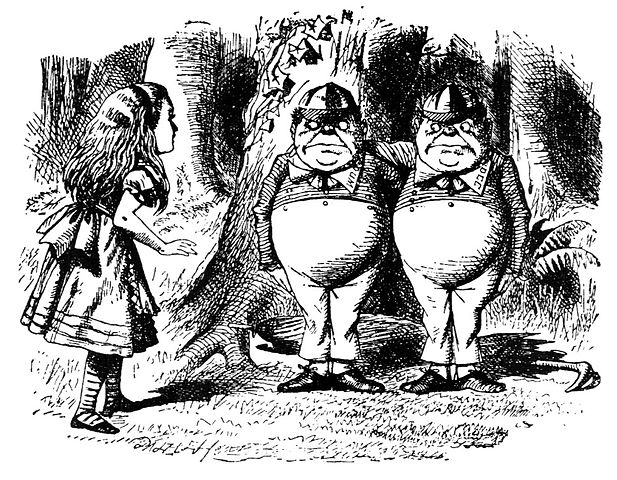
\includegraphics[width=0.5\linewidth]{img/tenniel-tweedle-dee-dum} \end{center}

\begin{epigraph}
`Contrariwise,' continued Tweedledee, `if it was so, it might be; and if
it were so, it would be; but as it isn't, it ain't. That's logic.'

---Lewis Carroll, Through the Looking Glass
\end{epigraph}

\textbf{\emph{Logic}} is the formal study of reasoning -- the attempt to justify or provide evidence for claims or beliefs. In this chapter we will look at the basic concepts and techniques for the logical analysis of arguments. As we will be seeing this will be useful in our discussions of ethics since much of what we will be doing will involve careful consideration of the justification of claims we make about ethics in general as well as particular topics in ethics.

\textbf{\emph{Before}} we get started though we need to clarify some terminology -- especially our use of the word ``argument.'' Too often this word conjures up a pointless verbal fight between people with opposed views. They argue rather than discuss because their differences of opinion are fixed in place and neither will budge. It is typically a good idea to stay away from arguments in this sense. The word argument as we are using it here, however, has quite a different meaning. For us arguments do not require differences of opinion because arguments are just attempts to explicitly provide back-up or justification for some claim that we might make. We offer arguments in this sense whenever we make the grounds for our belief explicit whether we are doing this within the confines of our own heads, in written form or spoken out loud whether or not anyone disagrees with us. Arguments in this sense of the term might appear in regular old verbal disputes. But as we will be seeing arguments are best looked at one at a time since each one stands or falls on its own merits.

\textbf{\emph{So, for philosophers,}} arguments are just attempts to provide support for whatever it is that we might claim is true. For example, maybe we think the death penalty is wrong, or the opposite, so we come up with an argument to show this. Or maybe we think that morality is a sham, nothing but a cover story for basically selfish motives. Once again, we can come up with an argument in support of this idea. Or on an even more abstract level we might think that moral judgments are just matters of opinion and that it is therefore a waste of time to even argue about what is right and what is wrong. Since none of these claims are self-evidently true (even though some people may think some of these are obvious) we'll need an argument to back it up, or at least to make explicit our reasons for claiming it. In the end, we can think whatever we want. That will, however, only get us so far -- either others will agree with us or not, and either it will be true or not. But we can also offer reasons in support of our claims in the form of arguments. As we will be seeing, not all arguments are equally persuasive, but there are clear cut and reliable ways of evaluating them to see which really provide the support we are after and which do not.

\hypertarget{arguments-rationality-and-rhetoric}{%
\section{Arguments, Rationality and Rhetoric}\label{arguments-rationality-and-rhetoric}}

\textbf{\emph{Arguments}} can of course be looked at as attempts to persuade other people that they should accept the claims that we are making. Because of this it may seem at first glance to be similar to rhetoric, also known as ``the art of persuasion.'' People who study and practice rhetoric often claim that rational argument is just one among many different methods of persuasion, appropriate at specific times, but not fundamentally different than other methods. That is, they claim that argument is a form of rhetoric. Philosophers, on the other hand, would like to insist on the basic difference between the two. Philosophers call attention to the fact that in rhetoric:

\begin{itemize}
\item
  Appeal is made to our emotions, prejudices, fears, hopes, etc. That is, who we are and what we feel about things matters. This is both its strength and its weakness.
\item
  Because of this, the persuasion that rhetoric produces doesn't last, once our feelings change, we are no longer convinced, and our feelings are constantly changing.
\end{itemize}

In rational argument, on the other hand:

\begin{itemize}
\item
  Appeal is made not to our emotions but to our ability to reason.
\item
  Since everyone is equally capable of reasoning, this means that arguments do not appeal to us personally. It doesn't matter who you are, a good argument should convince you.
\end{itemize}

\hypertarget{the-structure-of-arguments}{%
\section{The Structure of Arguments}\label{the-structure-of-arguments}}

\textbf{\emph{To see}} all of this more clearly, we need to take a look at how arguments work. But first things first -- we need a more precise definition of what we mean by an argument in the first place. That's easy enough:

\begin{rmdnote}
An argument is a series of statements where some of these statements are
intended to provide evidence or support for others. When we argue we are
attempting to establish some claims on the basis of other claims.
\end{rmdnote}

\textbf{\emph{As sets of statements}}, arguments involve the declarative use of language. Declarative statements (or propositions) are just sentences that state stuff, they make claims, and so they can be either true or false. So when we are looking at arguments we are deliberately ignoring the many other ways we can use language, such as asking questions, making commands, expressing feelings. When we are offering an argument we are making a series of claims in which some are supposed to provide support for others. The statements that are doing the supporting are known as \emph{premises}. The statement that is being supported, the point of our argument is called the \emph{conclusion}.

\textbf{\emph{It is, however,}} sometimes difficult to tell whether a set of sentences is an argument or not. Let us consider a few examples:

\begin{argument}
Parents should have the right to make decisions about their own
children's healthcare. Why should other people mess around in their
business? And please, let's keep the lawyers out!
\end{argument}

This may seem like an argument, so how can we tell for sure? Simply by checking whether this set of sentences is a set of statements where some are intended to provide support for others. So, how many statements are there here? Only one: the first sentence is a statement, the second is a question and the third is a command. In other words, even though this looks at first like an argument it is really just a single claim with no real argument given in support.

\textbf{\emph{What about}} the next example? How many statements are in these sentences? And do any of them really offer support for any of the others?

\begin{argument}
I am convinced that aliens are living among us and you should be
convinced as well.

I have really good evidence for this claim.
\end{argument}

Well this is almost an argument, but not quite. There is a claim being made here: aliens are living among us. But there is no real support given for this claim, only the insistence that this person has some unknown evidence. Before we can start to evaluate this evidence to see whether it really supports the claim, we need to see it. So here we have only two separate statements without a real argument yet.

\textbf{\emph{Now consider}} the following example:

\begin{argument}
Christopher Columbus was a criminal, because anyone who kills innocent
people, kidnaps others, and steals their valuables is a criminal and
that is just what he did.
\end{argument}

Here the grammatical form is a little misleading. This is an argument in spite of the fact that there is only one sentence. Why? Because this one sentence expresses a few different claims or propositions and some of these claims are offered as supports for others. We can see this if we break it up into individual claims and change the order around like so into \textbf{standard form} with the premises listed as individual statements and the conclusion below a line that can be read as meaning ``therefore.''

\begin{argument}
Anyone who kills people, kidnaps other people and steals their valuables
is a criminal.\\
Christopher Columbus did all of those things.

\begin{center}\rule{0.5\linewidth}{\linethickness}\end{center}

So Christopher Columbus was a criminal.
\end{argument}

Perhaps this is not yet a very convincing or complete argument, but at least it is an argument unlike the first examples.

\textbf{\emph{It is not}} always so clear which statements in an argument are the premises and which statement is the conclusion. Often, but not always, these are signaled with one of a number of typical words or phrases that function as premise or conclusion indicators. Paying attention to these typical words and phrases can help you to disentangle the argument from the peculiarities of a writer's style.

\hypertarget{premises}{%
\subsection*{Premises}\label{premises}}


\textbf{\emph{To help guide}} us through an argument a writer or speaker who is presenting an argument might use the following expressions and phrases to show what the argument rests on. These are \emph{premise indicators}.

\begin{rmdnote}
\begin{itemize}
\tightlist
\item
  Because
\item
  Since
\item
  In light of the fact that
\item
  In view of the following evidence
\end{itemize}
\end{rmdnote}

This is not an exhaustive list. Basically, when reading an argument you can pick out the premises by asking yourself where the writer is starting from and where he or she is going. The first is the set of premises and the second is the conclusion.

\hypertarget{conclusions}{%
\subsection*{Conclusions}\label{conclusions}}


\textbf{\emph{It is often}} the case that arguments are presented with the conclusion first in order to emphasize where the discussion is supposed to be going. The following common words are often used to indicate a statement that is supposed to play the logical role of the conclusion of an argument.

\begin{rmdnote}
\begin{itemize}
\tightlist
\item
  Therefore
\item
  It follows that
\item
  Thus
\item
  It should be clear that
\end{itemize}
\end{rmdnote}

These words and phrases indicate that this is where the writer (or speaker) is going with the argument and they are often used at the beginning of an informal argument to orient us, even though logically speaking they are last. For example, when a lawyer begins her argument in court with the claim, ``Your honor, ladies and gentlemen of the jury, my client is not guilty,'' and then goes on to present the evidence, she is reversing the logical order for rhetorical effect. This is fine in everyday life, but since it can be confusing, when we look at arguments explicitly here we will look at them in standard form with the premises first and conclusion last.

\hypertarget{pattern-of-reasoning}{%
\subsection*{Pattern of reasoning}\label{pattern-of-reasoning}}


\textbf{\emph{One other thing}} to watch for when looking at arguments is words and phrases that indicate the structure of the reasoning itself. These are ways of pointing out exactly how the premises are supposed to support the conclusion, and so are indicators of the pattern or form of reasoning involved. Some examples are:

\begin{rmdnote}
\begin{itemize}
\tightlist
\item
  Because of these, that has to be true.
\item
  If this then that, otherwise this.
\item
  All of the above is true so this means\ldots{}
\item
  This is the only option that makes sense.
\item
  If we assume that this is true we get a ridiculous result so it can't
  be true.
\end{itemize}
\end{rmdnote}

These indicate the general logic form of argument being followed. Is it a matter of necessity, other conditions present or absent, summation of influences, or a process of elimination, or are we showing something indirectly by showing that denying it makes no sense? The more formal study of logic looks carefully at these and many other different patterns of reasoning, and we will meet them at various points in our discussions of arguments about topics in ethics.

\hypertarget{validity-and-soundness}{%
\section{Validity and Soundness}\label{validity-and-soundness}}

\textbf{\emph{Not all arguments}}, however, are really equal. Just having any old argument won't always get us very far. Instead, as we will see, there are some arguments that really are better than others. This was the insight of the first philosophers in the Western tradition, Socrates, Plato and Aristotle, and it does seem kind of strange that I feel compelled to have to justify it even after a couple of thousand years. Way back then, just like now, many people thought this was a presumptuous claim to make. This is especially the case since it amounts to the claim that some arguments are really compelling on their own, and that we should, as long as we are being rational, have no choice but to accept them. For the skeptics out there who doubt that we will ever be able to create such an argument, I should also point out that the clearest and best arguments really don't end up saying anything very controversial or extraordinary. This is one of the limitations that logic imposes on us: if we are really being logical and using only reliable arguments we may have to refrain from claiming to be able to establish very much. Understanding the logic of arguments, if nothing else, should encourage us to be a little more modest in our claims to knowledge. And this is why Socrates, in spite of his reputation for being a bit of a jerk in pointing out to many people the flaws in their own arguments is today most well known for saying that the only thing he really knew what how little he knew.

\textbf{\emph{To get back to business,}} when we are arguing what we are doing is trying to establish the truth of something that we don't know on the basis of other things that we already know or accept. What we are interested in is establishing the truth of the conclusion, yet for some reason it's truth is not obviously apparent to us so we need to establish it on the basis of other claims the truth of which we can already accept. Arguments move us from the known to the unknown.

\textbf{\emph{To take}} a simple example, suppose we would like to establish that Socrates fears death. We don't have any direct reason for thinking that this is true. But we do know some other things that may be of use in establishing this. First we know that Socrates is a human being. Second we know that all human beings are mortal. Third, we know that all mortals fear death. In standard form this would be arranged like so:

\begin{argument}
Socrates is a human being.\\
All human beings are mortal.\\
All mortals fear death.\\

\begin{center}\rule{0.5\linewidth}{\linethickness}\end{center}

So Socrates fears death.
\end{argument}

This is a bit of a contrived example, but it can help us to see the key concepts we can use to evaluate any argument at all.

\hypertarget{key-concepts}{%
\subsection*{Key concepts}\label{key-concepts}}


\textbf{\emph{The information}} in the premises is enough information, as we can easily see, to establish our conclusion. Since Socrates is human he must be mortal, and he must fear death, since all mortals fear death. This argument seems like a pretty solid piece of reasoning. But how can we tell in general whether an argument is a good argument? It turns out that there are two questions we will need to ask about an argument in order to determine whether or not it is a good argument:

\begin{rmdnote}
\begin{itemize}
\item
  Is there a clear and solid connection between every step of the
  reasoning that leads us inevitably from premises to conclusion? In
  philosophical terminology: \textbf{is it valid}?
\item
  Are the claims that we started from, our premises, really true? In
  philosophical terminology: \textbf{is it sound}?
\end{itemize}
\end{rmdnote}

How do we answer these questions for the example above? It seems that there is in fact a clear and solid connection between what the premises are saying and what the conclusion is saying. In fact we already showed this above when showed that the conclusion necessarily follows from the premises. Technically this is a short and informal \emph{proof} of its strength as an argument, that is, of its validity. So the answer to the first question is, yes, it is valid.

\textbf{\emph{As far as}} the second question goes, however, we may have our doubts. Are all of the premises really true? Socrates is (or was) a human being -- he was one of the first philosophers. And all human beings are in fact mortal, at least as far as the evidence we have goes. But do we really know whether all mortals, past, present and future fear death? So here is the one small weakness of the argument. If we could be assured that this premise was true the argument would be completely convincing and would provide adequate backup for the conclusion. But it rests, unfortunately, on a weak premise, so it is not a sound argument. Since these two ideas are both very important for everything we'll be doing here and not so obviously obvious, here are some more explicit definitions:

\begin{rmdimportant}
The best arguments must be both **valid* and \emph{sound.}

\begin{itemize}
\item
  \textbf{Validity}: in a valid argument IF the premises are true the
  conclusion MUST also be true.
\item
  \textbf{Soundness}: A sound argument is a valid argument that also has
  TRUE premises.
\end{itemize}
\end{rmdimportant}

One thing to notice here is that the test for validity is entirely independent of the test for soundness. It is a little misleading, as we can now see, to ask whether arguments are either good or bad. More precisely, they can be:

\begin{itemize}
\item
  \emph{Valid and sound}: these are the best arguments, because the premises really establish the conclusion, and the premises are true -- hence the conclusion really is true.
\item
  \emph{Valid but not sound}: these are promising arguments that exhibit good logical form, but that rely on less than perfect information in their premises, and so are not completely solid.
\item
  \emph{Invalid}: these arguments are bad arguments since they do not establish what they claim to be establishing. All invalid arguments are automatically unsound, since sound arguments are a subset of valid arguments.
\end{itemize}

\hypertarget{more-examples}{%
\subsection*{More examples}\label{more-examples}}


\textbf{\emph{Learning how}} to identify valid arguments is important for a course in philosophical ethics, since the philosophical approach to ethics consists largely of the examination of arguments about ethical issues. And the best way to learn this is by practicing. Consider the following argument, conveniently written in standard form:

\begin{argument}
The earth is a rotating sphere moving around the sun.\\
We are all on the surface of the earth.\\
Anything on the surface of a moving object moves with that object.\\

\begin{center}\rule{0.5\linewidth}{\linethickness}\end{center}

So we are all moving around the sun.
\end{argument}

Forget for a moment about whether or not you buy the conclusion on its own. In analyzing an argument we need to know whether the premises support the conclusion adequately, so we pretend that we are not sure about the truth of the conclusion. Our first test is the test of validity. We ask ourselves: if the premises were true, could the conclusion be otherwise? Is the truth of the conclusion guaranteed by the truth of the premises? In this case it seems clear that if we are in fact all on the surface of an object that is moving around the sun, then we would all also have to be moving around the sun. So the argument is valid.

\textbf{\emph{Notice}} that establishing an argument's validity is not yet establishing that the conclusion is really true. It is only establishing that the conclusion would be true, if only we could show that the premises were true. In fact this argument was rejected until about 500 years ago because nobody was willing to accept the truth of the first premise. Establishing that this was true took quite a bit of effort by Copernicus, Kepler, Galileo and other early modern scientists. However, we now know that the premises are true. So this argument is not only valid, but also sound. And since it is sound we have proven beyond the shadow of a doubt that the conclusion is true. One more thing to point out here is that this argument has always been sound (or at least as long as the solar system has existed) even if many people denied the truth of the first premise. They were simply mistaken in this denial.

Let's look at another example:

\begin{argument}
If you want to see the world, you should join the navy.\\
Jane wants to see the world.\\

\begin{center}\rule{0.5\linewidth}{\linethickness}\end{center}

So Jane should join the navy.
\end{argument}

This argument is a little trickier because it contains an \emph{If \ldots{} then} statement. If \ldots{} then statements, also known as conditionals, make indirect claims. They don't just tell us what is the case, they tell us what would be the case if, or on condition that, something else were true. With this in mind let us consider this second argument. First we check for validity, by assuming that the premises are true and seeing if the conclusion would have to be true as well. In other words we are not yet interested in whether or not they really are true, but whether the argument works as an argument, whether the conclusion logically follows from the premises. It seems pretty clear that this argument is valid. This is because \emph{if}, as the first premise claims, the navy really is the best way to see the world, \emph{and if} as the second premise claims, a person named Jane wants to see the world, then she should clearly join the navy. Notice that this argument's validity does not have anything to do with its content, with the particular claims being made. Instead, validity is a matter of form, so that we could substitute any other content for the content of this argument without affecting its validity. Essentially this argument has the following form:

\begin{argument}
If A, then B.\\
A.\\

\begin{center}\rule{0.5\linewidth}{\linethickness}\end{center}

Therefore B.
\end{argument}

\textbf{\emph{Here}} A, B can be substituted by any statements we please, as long as our substitution is consistent throughout the argument. In all cases the resulting argument will turn out to be valid. Try it and you will see that the resulting arguments all come out valid. This is because validity is a matter of logical form regardless of the content we are arguing about.

\textbf{\emph{The soundness}} of arguments, however, unlike validity, has everything to do with content, because an argument is sound when it is valid and it \emph{also has true premises}. Back to the argument about Jane. Is it sound? First we note that it is valid, then we ask whether or not the premises are really true. Consider the first premise: ``If you want to see the world you should join the navy.'' It may be true that joining the navy is one way to see the world (provided that you don't end up on a submarine, or in the engine room of a ship), but is it the only way? Of course not, so the first premise is just false. The second premise is also questionable, but for a different reason -- we simply do not know who Jane is since this is a fictional example. So in spite of its validity this argument is unsound and we need not accept the conclusion as a true statement. It may in fact be true, but this argument gives us no good reason for thinking so. As an exercise you might want to try coming up with a sound argument that follows the form of this one.

\textbf{\emph{Now consider}} as our next example, the following argument:

\begin{argument}
If you want to see the world, you should join the navy.\\
Jane joined the navy.\\

\begin{center}\rule{0.5\linewidth}{\linethickness}\end{center}

So Jane wants to see the world.
\end{argument}

This argument seems similar to the previous one, but it has one important difference. The conclusion of this argument was the second premise of the last argument, and the second premise of this argument was its conclusion. What happens to the validity of the argument when we make this simple change? Notice what this argument is saying. It is offering an explanation of why it is that Jane joined the navy -- because she wanted to see the world. The question is, and this is the way we check for validity, are there any other possible explanations of why she joined the navy that are consistent with the premises? In other words, \emph{is it possible for the premises to both be true and the conclusion false}? The answer is yes. It all hinges on what the first premise doesn't say. It doesn't say that the only possible reason to join the navy is the desire to see the world. It just says that if that's what you happen to want then the navy is for you. So Jane could have joined the navy only because she wanted to learn all there is to know about marine diesel engines without caring whether she learned this in New Jersey or in the South Pacific ocean. To put this in yet another way: if it is at all possible, if there are no contradictions involved, for the premises of an argument to be true and the conclusion false, then the argument is invalid. This argument is invalid for precisely this reason. Furthermore, since it is invalid, this automatically makes it unsound, since in order for it to be sound it has to first be valid.

\hypertarget{proofs-and-counterexamples}{%
\section{Proofs and Counterexamples}\label{proofs-and-counterexamples}}

\textbf{\emph{Another}} way to look at the difference between valid and invalid arguments is in terms of the difference between a proof and a counterexample. A proof is a step by step demonstration that the conclusion is a \textbf{necessary} consequence of the premises. To prove that a conclusion validly follows from a set of premises we show in a detailed way how a series of obviously valid steps in reasoning lead us to the conclusion. Take the following argument for example.

\begin{argument}
Fred is older than Wilma but younger than Betty.\\
Barney is older than Betty.

\begin{center}\rule{0.5\linewidth}{\linethickness}\end{center}

So Barney is older than Fred.
\end{argument}

Remember that a valid argument is one in which \textbf{\emph{if}} the premises are true, the conclusion must also be true. So how would we prove that this is the case? Well we just \emph{assume} that the premises are true and go from there. So here is what a proof might look like:

\begin{rmdtip}
The first premise states that Fred is older than Wilma and he is younger
than Betty. Wilma doesn't matter here since she isn't mentioned in the
other premise or the conclusion, so let's just note that this premise
clearly states that Fred is younger than Betty. Now this would mean that
Betty is older than Fred, since ``older'' and ``younger'' are inverses.
If I am younger than you then you are older than me no matter who we are
since that's what ``younger'' and ``older'' mean. Now since Barney is
older than Betty, as the second premise states, he must be older than
Fred too, since as we just saw, Betty is older than Fred. This follows
from the fact that the relationship ``older than'' is a
\textbf{transitive} relationship -- if A is older than B and B is older
than C A has to be older than C since that's ``just what''older than"
means. So our conclusion that Barney is older than Fred is clearly a
\emph{logical consequence} of the premises.
\end{rmdtip}

\textbf{\emph{That's all}} there really is to any proof. We have just unpacked the meaning of what the premises are saying in a way that establishes that they entail the conclusion. We don't, in other words, have to add any new information to what is already stated in the premises in order to get the conclusion. In more complicated cases it can take much more effort to show this but all proofs are nothing but such a process of showing that the conclusion is thus ``contained'' in the premises already, which is of course \emph{why} the truth of the premises would guarantee the truth of the conclusion. In a simple case like this we can almost just see the obviousness of the connection between premises and conclusion, and so it might seem silly to spell things out in this much detail, but in more complicated cases there is more room for error so spelling things out like this is important.

\textbf{\emph{Invalid arguments}} in contrast are arguments where we would need something more than what is contained in the premises to get the conclusion. No matter how we attempt to prove our conclusion we will \emph{always} come to some spot where we cannot get any closer to the conclusion. So how do we show \emph{this}? We use a counterexample, which is nothing but a possible situation in which the premises would all be true and the conclusion would be false. This shows that the argument is invalid, since if it were valid it would be \emph{impossible} for the premises to be true and the conclusion false at the same time as we just saw. Consider the following argument:

\begin{argument}
Fred is older than Wilma but younger than Betty.\\
Barney is younger than Betty and older than Wilma.\\

\begin{center}\rule{0.5\linewidth}{\linethickness}\end{center}

So Fred is older than Barney.
\end{argument}

Even though we have no idea what these peoples' ages are (or even if they exist outside of a 1970's TV cartoon series) we can tell that the conclusion does not have to be true, even if the premises were true. This argument is invalid and we can show this with a counterexample.

\begin{longtable}[]{@{}cc@{}}
\toprule
person & age\tabularnewline
\midrule
\endhead
Barney & 36\tabularnewline
Betty & 40\tabularnewline
Fred & 35\tabularnewline
Wilma & 32\tabularnewline
\bottomrule
\end{longtable}

\textbf{\emph{Notice that}} if these people had these ages, this would make all of the premises true and the conclusion false. If Fred is 35, Wilma is 32, Betty is 40 and Barney is 36, then it is true that Fred is older than Wilma, but younger than Betty -- which is what the first premise claims. It is also true that, given these ages, Barney is younger than Betty and older than Wilma -- which is what the second premise claims. But Fred is not older than Barney. In other words, what these ages show that it is \emph{possible} for the premises to be true and for the conclusion to be false and thus that the reasoning involved in getting to the conclusion is invalid. Even if we had true premises, this would not be enough to guarantee the truth of the conclusion. That is what terrible reasoning is all about. We will many more examples of bad reasoning in the next chapter on logical fallacies.

\hypertarget{going-further}{%
\section*{Going further}\label{going-further}}


\begin{rmdslides}
For the slideshow summarizing the main points of this chapter,
\href{https://gwmatthews.github.io/ethics-slideshows/02-logic.html}{click
here}.
\end{rmdslides}

There is, once again a great many web sources that can help clarify the concepts covered in this chapter. Many are oriented towards programmers or computer scientists (computers are automated logic machines after all) and these can get very technical, very quickly. So here are a couple that are a bit more approachable.

\begin{itemize}
\item
  For a slightly different and more in-depth treatment of the basic concepts of logic see \href{https://jonathanweisberg.org/vip/logic.html\#logic}{the logic chapter} of Jonathan Weisberg's open source textbook on probability and statistics, \emph{Odds \& Ends.}
\item
  Wireless Philosophy is a well-produced series of short videos on a great many topics in philosophy. Their \href{https://www.youtube.com/playlist?list=PLtKNX4SfKpzX_bhh4LOEWEGy3pkLmFDmk}{playlist on Logic and Critical Thinking} is a great resource for exploring logical thinking in all of its complexity, 5 or 6 minutes at a time.
\end{itemize}

\hypertarget{fallacies-and-biases}{%
\chapter{Fallacies and Biases}\label{fallacies-and-biases}}

\begin{center}
\includegraphics[width=0.4\linewidth]{img/illusion} \end{center}

\begin{epigraph}
Reality is, you know, the tip of an iceberg of irrationality that we've
managed to drag ourselves up onto for a few panting moments before we
slip back into the sea of the unreal.

---Terence McKenna
\end{epigraph}

\textbf{\emph{Throughout}} our discussions of logic so far, you may all have been wondering how often anyone ever lives up to the standards of logical reasoning as we have laid them out here. It may seem fairly obvious that most people do not seem to be either willing or able to accept only those claims that are conclusions of sound arguments, but instead we often decide based on feelings and instincts or on the basis of what we just want or assume to be true at the outset. In fact, there is a theory of the origins of our capacity for logical reasoning known as the ``\href{https://www.edge.org/conversation/hugo_mercier-the-argumentative-theory}{argumentative theory of reasoning}'' that claims that our logical abilities, such as they are, evolved to enable us to ``prove'' ourselves right. Before the abstract study of logic was invented by Aristotle, who sought the universal principles governing reasoning, we were all already adept at persuading others by manipulating logic for the sake of convincing others that we were right and hence asserting social dominance, whether or not our claims were truly justified. It seems, in other words, that the rhetoricians were right after all that logic is just one means of persuasion among others, no better or worse than them, but maybe more or less effective in different contexts.

\textbf{\emph{Or is it?}} As we saw in the last chapter, there is something to be said for being logical. Put simply, valid and sound reasoning really just boils down to not saying more than you really know and this seems like a pretty reasonable approach if we want to figure out what is true and what is not. It is, however, abundantly clear that us humans often fail to abide by this principle and make claims that we really don't have much support for. This chapter explores two related ways we do this -- by committing fallacies and by getting caught by various ``cognitive illusions.'' Fallacies are bad arguments -- they are typically invalid -- that are often used to try to convince someone of some point that really has little argumentative support. They work, to the extent that they do, because they take advantage of certain weaknesses in our reasoning skills. As we will be seeing, a careful analysis of how various different forms of fallacious reasoning work and of what mistakes they make can provide us with a certain degree of protection from those who would use them to convince us of things that have little real support. Cognitive illusions are related in that they lead to mistakes in reasoning, but they are often more difficult to spot and avoid falling prey to, since they are mistakes rooted in mental shortcuts that can be reliable in certain contexts. Like visual illusions, they are false representations of reality, which, even if we know they are false, we cannot help falling prey to. Looking at some common cognitive illusions can help us to see, however, why we should sometimes not trust our own thought processes as much as we often do. And this as well can provide us with more tools for distinguishing between between what is really the case and what just seems to be so.

\textbf{\emph{As we turn to examine}} some important logical fallacies it is helpful to keep in mind that there are both many more particular fallacies than the ones we are going to look at and also many different ways of categorizing them. The thing to keep in mind here is that all stretch logical support beyond its breaking point, and how in particular this happens is not always so clear. On the other hand you can usually see the weakness of an argument that relies on a fallacy by asking yourself a simple question about it: What is being claimed here, and on the basis of what? This often reveals the basic weakness of the argument as it involves stepping back from the particular claims being made in order to see the broader pattern and strategy of reasoning involved. It is this pattern that is flawed, regardless of the content of the argument. As a result, we can often find instances of the same form of fallacious reasoning used with many different topics, especially those that are controversial.

\textbf{\emph{In addition}} it can be helpful to look at fallacies in terms of a few more general types of mistakes in reasoning. That is what we will do here as we examine some different forms of bad reasoning under the headings: \protect\hyperlink{relevance}{fallacies of \emph{relevance}} -- all of which rest reasoning or points that are really just not relevant to the discussion; \protect\hyperlink{ambiguity}{fallacies of \emph{ambiguity}} all of which depend on the ways in which many words and expressions can have multiple and often incompatible meanings; and \protect\hyperlink{presumption}{fallacies of \emph{presumption}}," which depend on unacknowledged, unjustified extra assumptions.

\hypertarget{relevance}{%
\section{Fallacies of Relevance}\label{relevance}}

\textbf{\emph{As we turn to}} the fallacies of relevance, it is good to remember, that this set of fallacies rests on the use of information that may seem relevant to establishing the conclusion but isn't really relevant at all. They often play on our emotional responses to certain situations and topics and they can be quite effective as means of persuading us. They work so well in getting us to buy into their conclusions in part because of the nature of the human mind -- even though we are capable of thinking about things coolly and logically, we often jump to conclusions on emotional grounds and then enlist our cognitive abilities merely to rationalize decisions and conclusions we have already made. Philosophers would encourage us to resist such impulses and to stop and think before jumping to conclusions. This can of course be quite challenging just because of the way in which our brains are wired -- the neural pathway between sensory input to motor and cognitive output is shorter in its trip through those parts of the brain that process emotions than it is through our higher cognitive powers. But still, whoever said leading an examined life was the easiest thing to do?

\hypertarget{appeal-to-authority}{%
\subsection*{Appeal to authority}\label{appeal-to-authority}}


\begin{rmdwarning}
My friend who is a scientist insists that global warming is not cause
for alarm, and for me that is a good enough reason to accept her
conclusion.
\end{rmdwarning}

\textbf{\emph{This fallacy}} is also known as ``appeal to inappropriate authority.'' Appealing to authority is a commonly used way of trying to convince people. But why do we find authorities believable in the first place? Because they are authorities? In this case we may wonder why they are considered authorities at all. On the other hand if they have something to back up their claims, why don't we just see for ourselves whether they are right or not?

\hypertarget{ad-hominem}{%
\subsection*{Ad hominem}\label{ad-hominem}}


\begin{rmdwarning}
There is no need to take that animal rights activist seriously.

\begin{center}\rule{0.5\linewidth}{\linethickness}\end{center}

After all, she also benefits from the use of animals -- notice her
leather shoes and fur mittens.
\end{rmdwarning}

\textbf{\emph{The name}} of this fallacy is a Latin expression meaning ``against the person.'' It is also known as the ``abusive fallacy,'' or ``personal attack.'' This very popular fallacy focuses on the personal inconsistency of the person giving the argument in an attempt to discredit their argument. People who use this strategy don't respond directly to their opponent's argument but bring up external reasons not to believe anything he or she says. This is clearly wrong since it is the argument that someone gives and its validity and soundness that should be our concern not the person from whose mouth that argument happens to be coming.

\hypertarget{popular-appeal-bandwagon-fallacy}{%
\subsection*{Popular appeal (bandwagon fallacy)}\label{popular-appeal-bandwagon-fallacy}}


\begin{rmdwarning}
The Romans were justified in slaughtering thousands of slaves.

\begin{center}\rule{0.5\linewidth}{\linethickness}\end{center}

After all it was a part of their culture and not many people objected.
\end{rmdwarning}

\textbf{\emph{This fallacy}} involves appealing to what most people or the majority of people think as a way of determining what is really true or really right. But as pre-civil rights segregation laws show -- what the majority wants or believes can very easily be wrong. The fallacy known as the ``appeal to tradition'' is similar in that it claims that tradition, the way people have been doing things for a long time, is a good enough basis for us to believe or act as they did. This, of course overlooks the possibility that they were wrong or had no good reason to believe or act as they did.

\hypertarget{appeal-to-force}{%
\subsection*{Appeal to force}\label{appeal-to-force}}


\begin{rmdwarning}
The reason that we are right is because we have the military might to
get rid of any government that disagrees.
\end{rmdwarning}

\textbf{\emph{However effective}} force or threats of force may be in getting people to do what we want, we may wonder whether this approach really is attempting to convince anyone of anything. Even though threats may get people to say that they agree with you, this shows nothing about whether or not the conclusion is true or whether they really believe what you are saying.

\hypertarget{appeal-to-consequences}{%
\subsection*{Appeal to consequences}\label{appeal-to-consequences}}


\begin{rmdwarning}
If astronomers are correct, the earth orbits a relatively insignificant
star in a remote corner of one galaxy among billions.

\begin{center}\rule{0.5\linewidth}{\linethickness}\end{center}

But this conclusion violates our sense of the significance of our own
lives and so it must be false.
\end{rmdwarning}

\textbf{\emph{This fallacy}} involves rejecting some particular viewpoint, theory or idea based on the consequences to which it leads. These consequences are often emotionally loaded, the kinds of things that we may not want to believe. However, it is often simply irrelevant whether or not we like or want to believe something: the truth may in fact be indifferent to what is pleasing to us. The way to tell what the truth of the matter is, is to examine the evidence rather than reject a theory out of hand because it has unappealing consequences.

\hypertarget{the-naturalistic-fallacy}{%
\subsection*{The naturalistic fallacy}\label{the-naturalistic-fallacy}}


\begin{rmdwarning}
Women alone are capable of having babies.

\begin{center}\rule{0.5\linewidth}{\linethickness}\end{center}

So the responsibility of raising and taking care of them is entirely
theirs.
\end{rmdwarning}

\textbf{\emph{Next we have}} the naturalistic fallacy. We often appeal to nature as if natural things, practices, etc. were automatically good. This is perhaps understandable in a world filled with various artificial substances of dubious safety. But we should be careful of making such appeals since they involve a leap of logic. The problem with the naturalistic fallacy is actually quite a general problem -- the attempt to conclude something about what should or ought to be be the case from what simply is the case. In this example, the facts of how human reproduction work entail nothing about who should play what role in raising children. That is a matter of social relations that, us philosophers hope, should be based on a free and open (and rational) discussion between those involved and not on the ``facts of life.''

\hypertarget{red-herring}{%
\subsection*{Red herring}\label{red-herring}}


\begin{rmdwarning}
We shouldn't worry that much about people dying of horrible diseases in
Africa.

\begin{center}\rule{0.5\linewidth}{\linethickness}\end{center}

After all we have problems of our own to deal with.
\end{rmdwarning}

\textbf{\emph{The name}} of this fallacy comes from the British method of fox hunting. First a captive fox is released and then a pack of foxhounds follow its scent trail, followed in turn by the hunters. In order to make it a little more difficult for the hounds to follow the fox, a piece of smoked herring (a smelly fish that typically is red in color) is wiped on the ground across the fox's path and thrown off to the side somewhere. This serves to distract and confuse the hounds and gives the fox a chance to get away. In an argument whenever you bring up something irrelevant in order to draw attention away from the topic at hand you are relying on the fallacy of red herring. The problem with the reasoning in this example, of course, is that there is no mention made of the possibility that both problems in Africa and problems here can be addressed. Besides mentioning something off the topic in no way undermines whatever claims are made about that topic.

\hypertarget{weak-analogy}{%
\subsection*{Weak analogy}\label{weak-analogy}}


\begin{rmdwarning}
Galileo was ridiculed because of his views, and these views later proved
to be correct.\\
I too am ridiculed for believing that the Pope is a reptilian alien in
league with the Freemasons.

\begin{center}\rule{0.5\linewidth}{\linethickness}\end{center}

Thus I too will have my day and my views will be accepted.
\end{rmdwarning}

\textbf{\emph{Analogies are}} comparisons between different things. We reason analogically when we argue that because one object or concept has a certain feature, other objects or concepts that are similar in certain respects will also have that feature. This is an important way in which we make sense of the world. However, it has its drawbacks. If we are not careful we can end up making analogies when they are not really there. This argument is based on a weak analogy because it is just not the case that all views that are ridiculed end up prevailing in the end. Some do, like Galileo's, but the reason was not inherent in their being ridiculed, but on their being based on good reasoning supported by evidence in the appropriate ways. And by the way, there really are people who believe that the Pope is a reptilian alien, just google it and see.

\hypertarget{ambiguity}{%
\section{Fallacies of Ambiguity}\label{ambiguity}}

\textbf{\emph{The next set}} of fallacies relies on the fact that many terms have multiple meanings. Switching between meanings without acknowledging that one is doing so is a way of making invalid reasoning look valid. Closer examination reveals arguments that do this to be weaker than at first glance. Here we will consider just two examples. Many more often appear in debates.

\hypertarget{equivocation}{%
\subsection*{Equivocation}\label{equivocation}}


\begin{rmdwarning}
People in jail are really free.

\begin{center}\rule{0.5\linewidth}{\linethickness}\end{center}

This is because if you can think whatever you want, then you are free
and people jail can certainly think whatever they want.
\end{rmdwarning}

\textbf{\emph{Equivocation}} is using multiple meanings of a word as if they were the same. We start out with one meaning of a word like ``freedom'' and end up with another meaning, in the attempt to fool the person who is listening to us that our reasoning is valid. Used car dealers sometimes use a tactic known as ``bait and switch'' that is similar to this --- they advertise great deals in the paper and then when you show up to their lot they have something else similar but not quite as good a deal that they offer you instead.

\hypertarget{straw-person}{%
\subsection*{Straw person}\label{straw-person}}


\begin{rmdwarning}
The senator who suggested cutting funding for the new Air Force attack
drone system really wants to leave us defenseless against our enemies.

\begin{center}\rule{0.5\linewidth}{\linethickness}\end{center}

Thus we should reject such cuts.
\end{rmdwarning}

\textbf{\emph{This fallacy}} often appears in the context of a debate in which one person misrepresents his or her opponent's view in order more easily, as with a person made of straw, to knock it down. This is a fallacy of ambiguity in that it relies on a superficially similar version of the view that is being attacked rather than the view itself. One can often ``win'' debates by using this strategy, but such victories are hollow in that they do not really engage with the real issues but only with caricature. If you really want to demonstrate that some view you are attacking is worthy of rejection, it is far better to rely on the ``principle of charity'' which involves presenting your opponent's view in as favorable a light as possible. If it still fails to withstand scrutiny, then perhaps you are wrong to reject it. he drawback, however, is that if you represent your opponent's views in a more fair and favorable light, your objections to them may themselves not hold up. But then again, that is only a drawback if you care more about winning debates rather than in figuring out what is really the case.

\hypertarget{cherry-picking}{%
\subsection*{Cherry picking}\label{cherry-picking}}


\begin{rmdwarning}
This study of 12 children clearly shows a link between childhood
vaccination and autism.

\begin{center}\rule{0.5\linewidth}{\linethickness}\end{center}

Thus vaccines cause autism.
\end{rmdwarning}

\textbf{\emph{This one}} is really no joke -- in fact the whole of the current scare about childhood vaccinations and autism was ``established'' by a single study of twelve children! The fact that the paper was retracted, and its author was barred from medical practice didn't matter since its influence only grew since the date of its publication. The logical mistake here is that of selectively reading the evidence in favor of your own hypothesis, or ``cherry picking'' the data to get the juiciest bits while ignoring anything that contradicts it. The other name for this fallacy, ``Texas sharpshooter'' refers to the related practice of proving your worth as a target shooter by first shooting random holes in the side of a barn, and then afterwards drawing your target around a cluster of holes so that it looks like you are a great shot. Is this done in Texas? Probably not, but whoever named it must have had a low opinion of Texans -- no offense intended and if you are from Texas, substitute your state of choice.

\hypertarget{presumption}{%
\section{Fallacies of Presumption}\label{presumption}}

\textbf{\emph{The third set}} of fallacies we will consider here are those that make presumptions, often in a hidden way. That is, they rely on hidden and unstated assumptions written, as it were, between the lines. This strategy, however, cannot withstand critical analysis since if we can get the perpetrator of such fallacies to acknowledge these hidden presumptions we can see them for what they are, mere assumptions without warrant.

\hypertarget{mere-assertion}{%
\subsection*{Mere assertion}\label{mere-assertion}}


\begin{rmdwarning}
Abortion is just wrong, and that is all there is to it.
\end{rmdwarning}

\textbf{\emph{This is}} the simplest and most obvious kind of bad reasoning. As the name implies, mere assertion involves simply stating what you want to establish without presenting any evidence whatsoever to support it. It is truly amazing how often people simply assert something that they may think is true without bothering to offer anything to support this assertion.

\hypertarget{begging-the-question}{%
\subsection*{Begging the question}\label{begging-the-question}}


\begin{rmdwarning}
You should become a Christian.

\begin{center}\rule{0.5\linewidth}{\linethickness}\end{center}

This is because the Bible says that if you are not a Christian you will
go to Hell.
\end{rmdwarning}

\textbf{\emph{This strange sounding}} name really applies to a very simple technique. Someone who begs the question is guilty of assuming what they are claiming to establish in their argument. In other words they put a disguised version of their conclusion in the premises of their argument. That is, they are not really arguing for what they claim to be arguing for. This is an example of a fallacy that is nevertheless a valid form of reasoning. The problem here is that we cannot just assume that the conclusion is true, as someone who uses this way of argument is in fact doing. Begging the question is not, of course, always so obvious. We can see that this is a case of begging the question when we realize that the only people who will be convinced by this argument are Christians. Why? Simply because nobody else will take evidence from the Bible seriously, and people who consider the Bible as authoritative are already Christians. This example also shows why begging the question is also known as ``preaching to those already converted.''

\hypertarget{appeal-to-ignorance}{%
\subsection*{Appeal to ignorance}\label{appeal-to-ignorance}}


\begin{rmdwarning}
The claim that the death penalty deters crime has not been established
with any certainty.

\begin{center}\rule{0.5\linewidth}{\linethickness}\end{center}

Thus it is clear that it does not deter crime.
\end{rmdwarning}

\textbf{\emph{The fact that}} something has not yet been proven to be true does not mean that it is false. It is just unknown! Yet this fallacy assumes that if we do not have proof of something then that thing must be false.

\hypertarget{false-dilemma-black-or-white-fallacy}{%
\subsection*{False dilemma (black or white fallacy)}\label{false-dilemma-black-or-white-fallacy}}


\begin{rmdwarning}
Either living organisms are products of blind chance or they were
deliberately designed.\\
But it makes no sense that something as functionally complex as a living
organism is the result of blind chance.

\begin{center}\rule{0.5\linewidth}{\linethickness}\end{center}

Hence they must have been designed.
\end{rmdwarning}

\textbf{\emph{The argument here}} rests entirely on an assumption that is not always so easy to see, the assumption that the alternatives stated are the only ones there are. If this were the case, then the argument would stand, but often other alternatives are simply not even mentioned. Hence the dilemma, or choice between two alternatives, is here a false one. In the example below, which is often used against the theory of biological evolution, the missing alternative is precisely what Darwin articulated in his book \emph{On the Origin of Species}, a theory which contains an element of chance but which is not reducible to the blind chance that this argument presumes is the only alternative to deliberate design.

\hypertarget{hasty-generalization}{%
\subsection*{Hasty generalization}\label{hasty-generalization}}


\begin{rmdwarning}
All three of my ex-wives always told me what to do.

\begin{center}\rule{0.5\linewidth}{\linethickness}\end{center}

This clearly shows that all women want to control us men all the time.
\end{rmdwarning}

\textbf{\emph{We may be tempted}} to conclude a lot from a single case, or a relatively small sample, but this is often merely a way to confirm our prejudices. If we really want to make sweeping generalizations, we'll have to gather a bit more evidence in less clearly biased ways than this.

\hypertarget{slippery-slope}{%
\subsection*{Slippery slope}\label{slippery-slope}}


\begin{rmdwarning}
If we legalize physician assisted suicide then everyone over sixty had
better watch their backs.

\begin{center}\rule{0.5\linewidth}{\linethickness}\end{center}

Once doctors get used to helping people with terminal illnesses die
comfortably, they'll find it easier to get rid of older people.
\end{rmdwarning}

\textbf{\emph{Slippery slope arguments}} are often used as a way of warning us of the dangers of allowing people to do something that is now forbidden. They say, in effect, if we allow someone to do this, then they'll have no reason not to do that, which is much worse. The name comes from the metaphor of an icy ski slope: if we are foolish enough to step onto the slope, without skis on of course, we'll end up uncontrollably sliding down to the bottom. The problem with this argument is that it claims that we must end up where the arguer claims we will, but the argument gives us nothing but the assertion that we will in fact end up there.

\hypertarget{false-cause}{%
\subsection*{False cause}\label{false-cause}}


\begin{rmdwarning}
The majority of heroin users smoked marijuana when they were younger.

\begin{center}\rule{0.5\linewidth}{\linethickness}\end{center}

So smoking marijuana must be one of the causes of heroin use.
\end{rmdwarning}

\textbf{\emph{Us humans}} are very good at noticing patterns in the world around us. In fact science is based on this ability -- we notice regularities and then come up with explanations for them. The most powerful of these explanations involve attributing a causal relationship between events that appear to be related to each other in a regular way. We have to be careful here, however, since we also have the tendency to overdo this. This may seem like a convincing argument until we recognize that the fact that something tends to happen before something else is not nearly enough to establish that the first thing causes the second to happen. For example, the fact that my alarm clock goes off every day shortly before sunrise does not mean that my alarm clock causes the sun to rise. The same goes for drug abuse. The fact that I abused marijuana first and then heroin later does not mean that the first caused the second. It is equally possible that I abuse whatever drugs I abuse for another reason -- I have major problems I am trying to escape from.

\hypertarget{circular-reasoning}{%
\subsection*{Circular reasoning}\label{circular-reasoning}}


\begin{rmdwarning}
He must be guilty, since he has a guilty look on his face.

\begin{center}\rule{0.5\linewidth}{\linethickness}\end{center}

Furthermore, the look on his face indicates guilt, because he is the one
who did it.
\end{rmdwarning}

\textbf{\emph{This final fallacy}} in our list is, in a sense, a more complex version of begging the question. Circular reasoning involves bouncing back and forth between two assumptions each of which is supposed to be the basis for the other. To see the circular structure of the reasoning exhibited here it may help to figure out which statement is the premise and which is the conclusion. In this example, at first glance it seems like the conclusion is ``He is guilty,'' and this seems to be based on the premise that ``He has a guilty look on his face.'' However, the fact that the look on his face indicates guilt is then supported by the assertion that ``He did it.'' Clearly we are moving around in a circle -- our premise supports and is supported by our conclusion. There is thus no real support for either and the whole structure is unfounded. This fallacy is also known as the ``vicious circle'' fallacy.

\hypertarget{cognitive-biases}{%
\section{Cognitive Biases}\label{cognitive-biases}}

\textbf{\emph{Fallacies}}, as we have been seeing, are common mistakes that we make in reasoning especially when we are trying to support a conclusion that we have insufficient evidence to support, ways in which we claim more than we really know. In recent years cognitive psychologists have also explored the ways in which not only get our arguments wrong, but also tend to get things wrong in our own thinking, how as Thomas Gilovich puts it in the title of his book \emph{How We Know What Isn't So}.\citep{gilovichHowWeKnow1991} That is, we have a tendency to fall prey to biases and mistakes in our own reasoning whatever it is that we may end up defending later in our arguments. In this section we'll look at some of the most important and relevant of these cognitive biases.

\textbf{\emph{In general}} we might classify these biases into two general types: ``hot biases,'' or motivated irrationality where our interests, emotional responses or visceral reactions to things influences our thinking process; and ``cold biases'' or unmotivated irrationality which are a result of certain mental shortcuts and routines we rely on even in situations where they do not really apply. Let's look at some examples.

\hypertarget{hot-biases}{%
\subsection*{\texorpdfstring{\textbf{Hot Biases}}{Hot Biases}}\label{hot-biases}}


\textbf{\emph{Hot biases}} are also known as examples of ``motivated irrationality'' because they involve bending our reasoning to suit our wants and desires. Our motivations may not always be clear even to us, so we may not realize that we are caught up in such biases. Luckily, however, there are steps we can take to avoid falling prey to them.

\hypertarget{confirmation-bias}{%
\subsection*{Confirmation bias}\label{confirmation-bias}}


\textbf{\emph{Confirmation bias}} is our often unconscious tendency to give more weight to evidence supporting our pre-existing beliefs or hypotheses and our tendency to downplay the significance of evidence against them. The result is similar to cherry picking but it may not be a deliberate attempt to mislead, but more of a product of other unconscious tendencies.

\begin{rmdwarning}
I keep seeing more and more evidence in favor of my hypothesis! What
about the evidence against it? Well that must be based on faulty data
collection.
\end{rmdwarning}

Given that we have a strong tendency to fall prey to this bias, what steps might we take to avoid it? For one, we can use various ``blind'' methods of data collection and analysis to protect our reasoning from the errors involving confirmation bias. Hence when scientific studies are done the scientists doing the study, who know which hypothesis they are testing can turn over the data to a neutral third party who does not know the hypothesis to evaluate. This way the results can be assured of corresponding to the standards of statistical analysis rather than simply reflecting the desires of the researchers to be proven right.

\hypertarget{group-think}{%
\subsection*{Group think}\label{group-think}}


\textbf{\emph{Just like}} our pre-existing beliefs can influence what we take the evidence to support, likewise with our connections to other people can do so. When someone in a group we identify with comes up with an idea we have tendency to give it more weight than in fact it deserves. A great example of this occurred during the Kennedy administration with the Bay of Pigs incident. The plan was to send a small group of armed anti-Castro Cuban soldiers to the Bay of Pigs in Cuba with the thought that that would be enough to incite a full-scale revolt against the Communist government by the rest of the Cuban population. Enough members of Kennedy's National Security Council which planned and approved the incursion were strongly in favor of it that they collectively ignored their own military intelligence which indicated that there was little popular support for revolting against the Cuban government. So when the invasion happened in January 1961 the initiative was quickly defeated and the Cuban exiles who landed in the beach were quickly arrested and imprisoned much to the embarrassment of the Kennedy Administration.\citep{BayPigsGroupthink}

\hypertarget{wishful-thinking}{%
\subsection*{Wishful thinking}\label{wishful-thinking}}


\textbf{\emph{These last two}} biases could be considered specific examples of a more general tendency we have towards wishful thinking, which is the tendency to project our own desires onto reality and fool ourselves into thinking that reality conforms to how we would like it to be.

\begin{rmdwarning}
I just know that the Yankees will win the World Series, they just can't
let me down again!
\end{rmdwarning}

All of these biases fail to make a distinction between what we would like to be the case and what really is in fact the case. We may end up lucky and happen to find out that reality conforms to how we would like it to be, but then again we may not. We can protect ourselves against these kinds of biases first by being aware of our own tendencies to fall prey to them and then by using particular strategies to separate our analysis of the evidence from our wishes.

\begin{center}\rule{0.5\linewidth}{\linethickness}\end{center}

\hypertarget{cold-biases}{%
\subsection*{\texorpdfstring{\textbf{Cold biases}}{Cold biases}}\label{cold-biases}}


\textbf{\emph{Cold biases}} differ from hot biases in that they are not such much results of our desires but of the ways in which our cognitive systems work. They are more like ``bugs'' in our mental operating systems than ways in which we twist our thoughts to conform to our desires.

\hypertarget{anchoringframing-effects}{%
\subsection*{Anchoring/framing effects}\label{anchoringframing-effects}}


\textbf{How much} are you willing to pay for some given product or service? Well it turns out to depend not just on the features of that product or service itself but also by what is next to it on the shelf, what other options you are presented with and even the initial asking price. These are examples of the ways in which the context of our choices influences the content of our choices. Many examples of this can be found in the marketplace. Here is just one example:

\begin{rmdwarning}
Today only, you can get a new Toyota for 20\% off the sticker price! So
act now and drive your new car away today!
\end{rmdwarning}

There are numerous ways in which advertisers and salespeople try to influence our choices. First the ``sticker price'' may or may not reflect anything about the reality of the product in question but may be intentionally inflated to anchor our minds to a price higher than we would actually pay. It turns out that doing so will make us more willing to pay a higher price than we would if the original non-discounted price were set closer to what we might actually pay, or what the manufacturer expects us to pay. Likewise, adding extra options that we may not actually be interested in independently can influence our willingness to buy a product, especially when it is compared to an otherwise equivalent product without those potions. In both cases our ability to compare what is offered with what we want is corrupted by the context within which the product is presented.

\hypertarget{the-fundamental-attribution-error}{%
\subsection*{The fundamental attribution error}\label{the-fundamental-attribution-error}}


\textbf{\emph{When it comes to}} explaining human behavior, and trying to figure out the relative weights of internal factors such as needs, desires and the personality of the actor on the one hand, and external situational factors on the other hand it turns out that we come up with different weights when thinking about our own behavior and that of other people. our own and others. We tend, for example, to put more weight on things outside of our own control when accounting for our bad behavior than we do when accounting for the behavior of others.

\begin{rmdwarning}
The fact that I tripped when walking down the street was because the
sidewalk was uneven. When you trip on the other hand, it's evidence that
you are a klutz.
\end{rmdwarning}

\textbf{\emph{In other words}} we are more generous with ourselves in terms of getting ourselves off the hook --- it's not my fault it's the situation I was in --- than we are with others --- clearly it is their fault! This is true that in many, many cases, if we looked at things in the more neutral terms of finding what factor most influence all of our behavior situational or external factors often play a much greater role than we think. So we are more accurate when we reflect on ourselves than when we look at the behavior of other people. Our attribution of causal influences tends to be skewed in the wrong direction when we look at why others do what they do especially when we compare it with our understanding of what influences us ourselves.

\hypertarget{the-availability-heuristic}{%
\subsection*{The availability heuristic}\label{the-availability-heuristic}}


\textbf{\emph{Finally}} in this brief survey of some major cognitive biases we have the confusion we tend to make between how readily something comes to mind (its ``salience'') and the more objective probability of its occurrence (its ``frequency''). Thus because terrorist attacks are so dramatic and stand out in our minds much more than the more common and mundane threats we are exposed to we tend to be more afraid of terrorism than, for example, driving to the airport. In the aftermath of the 9/11 attacks I remember listening to an interview with an expert on national security threats. The interviewer asked him what we could all do to be safer in international air travel and his response was ``Drive very carefully to the airport.'' This effect, once you start to notice it, is everywhere. We focus on dramatic if also highly unlikely threats and events and ignore those that are far more likely and hence, paradoxically, not so obvious to us.

\textbf{\emph{In this}} and the last chapter we have taken a closer look at what is involved in the justification of any claim at all. We have seen that the best arguments are both valid and sound -- they work logically in that their premises really provide adequate support for their conclusions and their premises are actually true. We have also examined some of the many mistakes in reasoning to which we are prone. These mistakes are not only used in a deliberately misleading way, since all of us have a tendency to make decisions and judgments first and then come up with reasons in support of them later. Thus we often rely on fallacious reasoning to rationalize our own beliefs or we tend to read the evidence is biased ways. As we will be seeing, as we turn now to start examining some of the many different theoretical approaches to ethics, the tools of logic and critical thinking will prove very useful in trying to come up with a reasonable answer to the general question, ``what is the right thing to do?''

\hypertarget{find-out-more}{%
\section*{Find Out More}\label{find-out-more}}


\begin{rmdslides}
Here is a
\href{https://gwmatthews.github.io/ethics-slideshows/03-fallacies.html}{summary
in slideshow form} of the content of this chapter.
\end{rmdslides}

\textbf{\emph{There are many}} great websites that list, discuss and explain the many ways we get things wrong in our thinking. Here are a few of my favorites.

\begin{itemize}
\tightlist
\item
  \emph{Your Fallacy Is} is a nicely designed website with more examples of common fallacies.

  \begin{itemize}
  \tightlist
  \item
    \url{https://yourlogicalfallacyis.com/}
  \end{itemize}
\item
  \emph{Your Bias Is}: is the sister site to Your Fallacy Is and focuses on common cognitive biases.

  \begin{itemize}
  \tightlist
  \item
    \url{https://yourbias.is/}
  \end{itemize}
\item
  Dan Ariely is a behavioral economist who studies human irrationality and has written a number of very readable books documenting his findings. He also has a number of videos of talks he has given on his site, \href{http://danariely.com/}{danariely.com}

  \begin{itemize}
  \tightlist
  \item
    \url{http://danariely.com/}
  \end{itemize}
\item
  And you should of course follow the \href{https://twitter.com/fallacy_ref?lang=en}{Logical Fallacy Ref} on Twitter.

  \begin{itemize}
  \tightlist
  \item
    \url{https://twitter.com/fallacy_ref}
  \end{itemize}
\end{itemize}

\begin{center}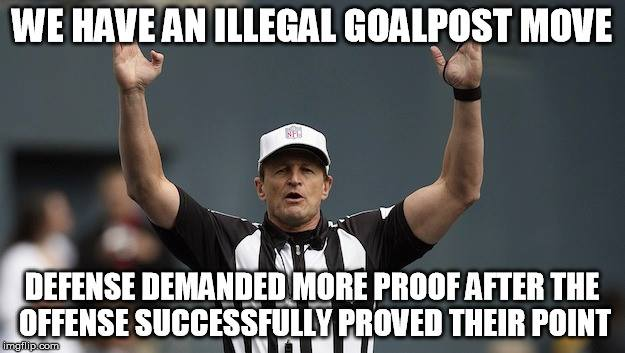
\includegraphics[width=0.6\linewidth]{img/fallacy-ref} \end{center}

\hypertarget{part-approaching-ethics}{%
\part*{Approaching Ethics}\label{part-approaching-ethics}}


\hypertarget{relativism}{%
\chapter{Relativism}\label{relativism}}

\textbf{\emph{Opinion}}, this seems to be where ethics starts and in many people's minds where it ends. You have a right to your opinion about right and wrong and I have a right to mine, so let's just leave it at that. Given what we have been looking at so far, not to mention all of the unread pages still ahead, it is probably already apparent that that is not going to be the whole story about ethics. It is nevertheless a deeply rooted assumption that ethical claims \emph{must be} opinions, since they are clearly \textbf{not} factual claims and that seems to be the only other sort of claim we can possibly be making when we are using language to state things. That this assumption does not in fact hold up to closer inspection is what this chapter is going to argue. Before we get to that argument, however, I would like to say a few words about what we are going to be up to in the next few chapters that make up this part of the text.

\textbf{\emph{In this part}} of the text we consider a variety of approaches to ethics. We'll start out from the approach that claims that ethics is just a matter of opinion. This is known as relativism and, in spite of its flaws as an account of ethics, it remains popular. Next we will look at two different variants of a claim that seems to be diametrically opposed to relativism -- the claim that ethics can and should be based on religion. And finally, we will examine a view that itself seems to swing back in some other direction, which again seems diametrically opposed to the attempt to root ethics in religion. This is known as egoism and it claims that ethics is psychologically or politically a dangerous and mistaken idea. In spite of the differences of these approaches, they do however share something in common, namely, the idea that if ethics is to make any sense at all our talk about ethics has to be translated into talk about something else like culture, or religion or psychology. As we will see none of the approaches we examine in this part of the text are ultimately adequate -- they all fail to capture what is distinctive about ethics and why ethical norms demand our attention. Thus in the third part of the text we will explore a range of philosophical attempts to reconstruct ethics on its own terms, to make explicit the basis for ethics as an independent source of norms.

\hypertarget{claims-and-consequences-of-moral-relativism}{%
\section{Claims and Consequences of Moral Relativism}\label{claims-and-consequences-of-moral-relativism}}

\begin{epigraph}
If anyone, no matter who, were given the opportunity of choosing from
amongst all the nations in the world the set of beliefs which he thought
best, he would inevitably -- after careful considerations of their
relative merits -- choose that of his own country. Everyone without
exception believes his own native customs, and the religion he was
brought up in, to be the best.

---Herodotus, The Histories
\end{epigraph}

\textbf{\emph{One of the}} most obvious facts to any casual observer of human behavior is its enormous diversity. People live in almost any conceivable physical environment, from dense tropical jungles, to frozen polar deserts, from small villages with thatched huts to modern industrial cities made of concrete, steel and glass. In addition, our cultural practices and norms reveal perhaps an even greater diversity. Some human cultures place value on devotion to the group at the expense of individual liberty, others emphasize the unique individual while downplaying our relation with others. Some cultures value continuity and tradition (think of the Amish of Central Pennsylvania) while others value innovation and rapid change (think of the Japanese fascination with technological innovation, for example the development of humanoid robot companions for older people). Some cultures value constant productive work while others place far more emphasis on living well and enjoying social interaction with others. Some cultures allow men and women to participate equally in all areas of social life, while others have entirely separate spheres for the two sexes. Recognition of this diversity is what has led some philosophers and social scientists to formulate a theory known as ``cultural relativism,'' which takes these casual observations and turns them into an explicit set of claims about the nature of value judgments. This theory is not only a popular theory about the nature of values. It also presents a challenge to the whole enterprise of philosophical ethics since it leads to the view that rational discussion and argument have little role to play in ethical decision making. Ethical decisions, opinions and judgments, according to cultural relativism, are always relative to the cultural environment within which they are made.

\textbf{\emph{Cultural relativism}} is one particular variant of a broader position that we can call moral relativism. Another variant is ``subjective relativism'' which appeals to individual feelings as the basis of moral judgment. Cultural relativism boils down to a few simple and seemingly obvious claims:

\begin{rmdnote}
\textbf{According to relativism}

\begin{itemize}
\tightlist
\item
  Ethical or moral claims are not objective in the way factual claims
  are.
\item
  There is no neutral standard for determining right or wrong.
\item
  All value judgments are relative to our personal or cultural
  perspective.
\end{itemize}
\end{rmdnote}

\hypertarget{a-first-case-for-relativism}{%
\subsection*{A first case for relativism}\label{a-first-case-for-relativism}}


\textbf{\emph{At first}} this set of claims may seem obviously true. After all, given the diversity of human values and customs, how could there be anything more than relative standards, standards that are only applicable within a given culture? Many people find relativism intuitively appealing and might even offer as a preliminary case for relativism the following points:

\begin{itemize}
\tightlist
\item
  \emph{Cultural diversity}: Human culture has always been extremely diverse. And many people seem to have equally diverse views on what sort of behavior is acceptable. It seems to follow from this that there cannot possibly be any standards for deciding between these views.
\item
  \emph{How we learn about values}: It seems obvious that we learn about values, and come to accept the values that we do because these are the values that are shared by the people who raise us. They are the values of our families and communities.
\item
  \emph{Intolerance}: There have been plenty of cases throughout history in which one group of people firmly believed that their values were not just acceptable for them but absolutely right, and used this as a justification for committing atrocities against other people. Relativists insist that the only way to avoid this kind of intolerance is to accept that there are no ultimate standards.
\end{itemize}

\hypertarget{what-is-at-stake}{%
\subsection*{What is at stake}\label{what-is-at-stake}}


\textbf{\emph{In a moment}} we will consider each of these points in greater detail. Before we do this it will be helpful to spell out what is at stake here. That is, we should consider what would be the case about ethical principles and decision making if cultural relativism were true. Its defenders make much of the positive consequences of this theory, while its opponents emphasize its negative implications. As we consider these consequences of the theory we must remember that whether or not we like where a theory leads us, in terms of its theoretical consequences, cannot itself determine whether the theory itself is correct. Reality does not care whether or not we like it. In the case of relativism at least, the extreme nature of its consequences helps explain why it is such a controversial theory.

\textbf{\emph{Defenders of relativism}} present it as the best way to acknowledge the great variety of human value systems and cultures. If there are no ultimately correct moral principles, then all human cultures become equally valid as ways of life, at least for different groups of people. This seems to encourage tolerance of other ways, a welcome relief after millennia of people intolerantly fighting with each other over their different views. After all, if there are no ultimate standards for right and wrong, we would could never justifiably say, ``Your group is wrong in doing what you do and so we have the right to force you to change your ways.'' On the other hand, a relativist cannot really consistently promote tolerance -- otherwise she would be granting tolerance for other cultural practices the status of a universal value, valid for everyone and this is what relativism says does not exist. So we should really say that relativism really only rules out one possible way of dealing with conflicts: the rational settlement of differences with reference to some kind of universal principles or values. Sometimes differences of opinions might be tolerated by the members of the groups that differ, sometimes one group will attempt to push its values on the other group. Both approaches are consistent with the claims of relativism.

\textbf{\emph{The first}} troubling consequence of relativism is one you may already have suspected: if there are no real standards, standards about right and wrong that are independent of cultural perspectives, it doesn't seem possible to condemn other cultures or individuals for doing awful things. For example, imagine that there is a society that has two major groups of people. One of these groups, who happen to be the majority of the population, decides that the other group doesn't deserve any respect, perhaps even that they are somehow naturally deficient or inferior. As a result they perform painful and often fatal experiments on the minority group, force them to work without pay, and even decide just to kill them off because it makes them feel better about themselves. What would a relativist say about this? It seems that since the relativist is only willing to recognize local or relative standards, she would have to conclude that although she doesn't like it, or that such behavior would never be tolerated in her society, she really can't condemn what this group of people are doing as simply being wrong. Why not? Well, because it seems right to the majority of people in that other society.

\textbf{\emph{Furthermore}}, relativism, if it were true, would require us to reject the idea that we can really make moral progress. Consider voting rights for women and African-Americans. In early American history both groups were denied these rights. Later on, after the Civil war in the case of African-American men and then in the early twentieth century in the case of all women, the Constitution was amended when people recognized that it was wrong to restrict these groups' access to the political process just because of race or gender. Many of us would consider this a case of moral progress -- a basic right was extended to people who had previously, for no good reason, been denied this right. What would a relativist say? Could they say that this was really a case of progress? Probably not, since progress implies that things are getting better, and this requires that there is some standard against which we can measure better or worse. So, for the relativist there is no progress, only different ways of doing things, none of which are really better or worse than any others. Is this a conclusion you are comfortable with?

\textbf{\emph{Relativism seems}} like a plausible theory about the nature of value judgments. It also seems, at first glance at least, to be a theory with nothing but positive implications -- it seems to encourage of diversity and lets everyone do their own thing. However, as we have just seen this easy-going character of relativism soon reveals a darker side. A relativist cannot really have any grounds for condemning any behavior at all, no matter how intuitively awful it seems, as long as someone believes that it is OK. In addition relativism does away with one of the most important parts of our moral thinking, the idea that maybe through our efforts we can make things a little better. This idea of progress is rendered simply meaningless by relativism. These implications of relativism do not by themselves let us know whether or not relativism is true. At best they reveal what the stakes are -- if relativism is true we get tolerance at the expense of having to tolerate anything all at that someone feels is the right thing to do. To determine whether or not relativism is true we need to consider more explicitly the arguments in support of this theory.

\hypertarget{defending-relativism}{%
\section{Defending Relativism}\label{defending-relativism}}

\textbf{\emph{Thus far}} we have been looking at the pros and cons of accepting relativism as an approach to ethics. In doing so we have been avoiding asking a simple question, that we now cannot any longer avoid -- \emph{is relativism true?} To answer this question we need to take a look at how we might argue for relativism instead of just leaving it as one opinion among others that we might take or leave. Although it may seem obvious to many people that relativism is in fact true, our examination of the explicit case that can be made in defense of relativism will show that it is not in fact based on very good arguments. But I am getting ahead of the story\ldots{}

\hypertarget{cultural-differences}{%
\subsection*{Cultural differences}\label{cultural-differences}}


\textbf{\emph{The first}} and most obvious way to defend relativism is based on the recognition of human cultural diversity. This was what motivated Herodotus to pronounce that ``custon is the kinf of all,'' and that has led many athropologists and sociologists to embrace it as well. So the first argument for relativism that we will examine here rests on recognition of the diversity of value judgments and tries to argue from this premise directly to the conclusion that there are no ultimate standards for right and wrong.

\begin{argument}
We all have different views about right and wrong.

\begin{center}\rule{0.5\linewidth}{\linethickness}\end{center}

Thus there are no standards about what is really right or wrong.
\end{argument}

\textbf{\emph{This argument}} may seem to be persuasive. Doesn't the fact of human diversity automatically entail relativism? But the question we should ask about this argument is not ``Does it seem persuasive?'', but ``Is it valid and sound?'' Remember a valid argument is one in which if the premises are true the conclusion must be true. So is this valid? How can we tell? We just ask, ``If the premise were true, would the conclusion also have to be true?'' In this case the premise seems obviously true, but does that by itself force us to accept the conclusion? Clearly not, since even if the premise is true and we do all disagree, this alone does not have to mean that there are no standards. However implausible it may seem that there are universal moral standards, the fact of human disagreement about what those standards might look like is just not enough to rule out the existence of standards. To see this, it may help to consider a clearly bad argument of exactly the same logical form in which the premise is clearly true and the conclusion is clearly false.

\hypertarget{a-counterexample}{%
\subsection*{A counterexample}\label{a-counterexample}}


\begin{rmdwarning}
We all have different views about how to deal with stop signs -- some of
come to a complete stop while others only slow down.

\begin{center}\rule{0.5\linewidth}{\linethickness}\end{center}

Thus there are no standards regarding stop signs.
\end{rmdwarning}

\textbf{\emph{The premise}} in this argument is clearly true as any casual observation of drivers at intersections will show. Yet the conclusion is also clearly false, since there really is a correct way to deal with stop signs, the one written in the relevant section of the laws governing driving. What this shows about the argument from cultural differences is that disagreement alone is not enough evidence for the conclusion that there are no real standards. From the fact that we may disagree about some topic we cannot conclude anything about whether or not any of us are really right or really wrong. We need much more evidence than this to support the conclusions of relativism. We disagree about many things. In some of these cases there is a way of settling disagreements -- look up the law, check the facts if we disagree about the temperature outside or whether or not it is still snowing. In other cases, there is simply no way to settle differences -- some people will just not be convinced that the Backstreet Boys or horrible musicians, or that sushi is the best dish on the planet. Likewise in all matters of style and taste.

\textbf{\emph{So this argument}} for relativism is inconclusive. Relativism focuses on our differences of opinion and tries to draw from this a conclusion that just does not follow. We still are no closer to deciding whether, as in cases of dispute about the law, we will be able to settle our ethical differences, or whether, as in cases of dispute about taste, we will not. It remains an open question whether or not there are standards in ethics.

\hypertarget{learning-right-from-wrong}{%
\subsection*{learning right from wrong}\label{learning-right-from-wrong}}


\begin{argument}
If we get our values from our cultural environments then our values are
culturally determined.\\

If values are culturally determined then they are relative to
cultures.\\

We do in fact get our values from our cultural environments.

\begin{center}\rule{0.5\linewidth}{\linethickness}\end{center}

Thus relativism is true -- values are relative to cultures.
\end{argument}

\textbf{\emph{This is a valid argument}}, so at first it seems like the relativist position might be stronger than we have be claiming. The question then becomes whether or not it is sound. Are the premises in fact true? The key premises are the first and the third. Let us consider the first: ``If we get our values from our cultural environments then our values are culturally determined.'' There are two ways we might understand this statement one of which makes it true by definition and the other of which makes it just plain false. If getting our values from our cultural environments means the same thing as our values being culturally determined, then the first premise is true, but completely uninformative, since it gives us no new information. But if, on the other hand, this claim is not true by definition it is in fact false, since it just does not follow that where we get something in any way determines what that thing is. As a counterexample: just because we learn arithmetic within the particular cultural environment of modern school systems does not mean that the content of arithmetic is at all determined by this environment. 2 + 2 = 4 wherever you happen to learn this. What we learn is at least in principle independent of where we learn it.

\textbf{\emph{The third premise}}, ``We do in fact get our values from our cultural environments,'' is equally suspect. It is possible that this is true, but it assumes some things about human psychological development that are simply unknown at this point in time -- the extent to which the ideas that we have in our heads are products of our immediate environments, and the extent to which they are products of built in psychological capacities and functions. Well then, where would ideas about right and wrong they come from, if not from the environment in which a person is raised? One possibility is that human moral development is somewhat built in, that we are all born with the capacity for social interaction and that this gets switched on, in a sense, as we grow and interact with others. If this view were correct we would expect to find that the variation of moral ideas among is humans is less pronounced than relativism claims. And in fact, if we ignore the surface differences between human value systems and look at the core values people accept, they start to look very similar.

\textbf{\emph{In fact}} we could take this point further and point out that all human cultures share certain basic values. We all:

\begin{itemize}
\tightlist
\item
  honor the dead with some sort of funeral rites and find it incredibly offensive to mistreat the dead.
\item
  act so as to help the group to survive.
\item
  believe in the importance of telling the truth in general, even if exceptions are sometimes made to this. distinguish between acceptable and wrongful killing of other human beings.
\end{itemize}

\hypertarget{saying-different-things}{%
\subsection{Saying different things}\label{saying-different-things}}

\textbf{\emph{Relativism isn't quite finshed}} yet though, since there is another popular argument in its favor that we haven't yet considered. This argument appeals to the, once again seemingly obvious, difficulty in coming to any kind of agreement about the meaning of basic moral terms.

\hypertarget{questioning-relativsm}{%
\section{Questioning relativsm}\label{questioning-relativsm}}

\textbf{\emph{The possibility}} that there is a common moral ground between groups of people is tempting as a possible alternative to relativism. What relativism gets right is the fact that we all disagree about how to carry out the basic moral demands these core values impose on us. But what it gets wrong is the degree to which we do all disagree. After all, we all have some way of honoring the dead, we all think that the survival of our group is important, we all recognize that communication is only possible against a general background of truth-telling, and we all agree that there is something that should be considered the wrongful killing of a human being or murder, even if different cultures have very different ways of putting these values into practice.

\begin{rmdcaution}
\textbf{\emph{But then}}, wait a moment, doesn't relativism just
reappear on another level? So what if we all agree on the importance of
honoring the dead? Our different views about how exactly to do this have
the potential to lead to serious conflict. And it is far from clear that
this kind of conflict, conflict about the implementation of core values,
can really be resolved.
\end{rmdcaution}

\textbf{\emph{In response}} to this problem let us take a closer look at what I claimed above was one of the common core values all human cultures share, the distinction we all make between acceptable and wrongful homicide. The relativist might argue that the fact that we all agree that there is such a distinction in all societies does nothing to alleviate the conflicts between societies. Take the way in which this value was put into practice in Nazi Germany: it was considered wrong to kill a member of the ``Aryan'' race, but acceptable and even necessary to kill Jews, Slavic people and Gypsies (among others). We, on the other hand, fought against Germany in WWII because, among other reasons, we disagreed that this was a legitimate way to make the distinction between acceptable and wrongful homicide. Our beliefs are that it is only acceptable to kill others in self-defense, in a just war or, in some cases, as a penalty for very serious crimes. Is there any way to resolve this conflict, or does relativism gain back all of the ground it has lost in the preceding discussion?

\textbf{\emph{Once we recognize}} that even Nazis are not living in a completely foreign moral universe, that they share with us the basic idea that there is an important moral distinction between justified and unjustified homicide, we can take a critical look at their way of making this distinction. And in fact it is quickly apparent that they made this distinction in a faulty way -- based on pseudo-scientific theories of race, based on the political manipulation of people's fears and based on paranoia. Hence, even on their own terms, the way in which they made this important distinction fails to be satisfactory. It is the fact that we share this basic distinction with them that enables us to criticize their way of putting in into practice. We can always ask of a given cultural practice or value, whether it is based on claims that stand up to scrutiny and whether it performs as advertised. This sort of internal criticism is only possible on the basis of shared human concerns that transcend different cultures.

\hypertarget{further-exploration-1}{%
\section*{Further exploration}\label{further-exploration-1}}


\begin{rmdslides}
Soon there will be a link here to the slideshow summary covering the
main points of this chapter.
\end{rmdslides}

\textbf{\emph{Relativism is}} a challenging position to take about ethics. It challenges its defenders to come up with an argument in favor of it that doesn't either \protect\hyperlink{begging-the-question}{beg the question}, or undermine itself.

\begin{rmdquestion}
Can a relativist ever lay claim to being correct about anything
including the correctness of relativsm? In case she did, then anyone
else could simply say, "well relativism may be true for you, but it's
not true for me!
\end{rmdquestion}

It is also challenging to its opponents since it seems to fit in well with the intractability of ethical stances. People \textbf{do} tend to dig in and refuse to either accept reasons against their own favored views or even the possibility of compromise.

\hypertarget{religion-and-ethics}{%
\chapter{Religion and Ethics}\label{religion-and-ethics}}

\hypertarget{divine-command-theory}{%
\section{Divine Command Theory}\label{divine-command-theory}}

\hypertarget{a-nasty-dilemma}{%
\section{A Nasty Dilemma}\label{a-nasty-dilemma}}

\hypertarget{natural-law-theory}{%
\section{Natural Law Theory}\label{natural-law-theory}}

\hypertarget{human-nature}{%
\section{Human Nature?}\label{human-nature}}

\hypertarget{egoism}{%
\chapter{Egoism}\label{egoism}}

\hypertarget{whats-in-it-for-me}{%
\section{What's in it for me?}\label{whats-in-it-for-me}}

\hypertarget{psychological-egoism}{%
\section{Psychological Egoism}\label{psychological-egoism}}

\hypertarget{ethical-egoism}{%
\section{Ethical Egoism}\label{ethical-egoism}}

\hypertarget{capitalism-and-the-common-good}{%
\section{Capitalism and the common good}\label{capitalism-and-the-common-good}}

\hypertarget{part-reconstructing-norms}{%
\part*{Reconstructing Norms}\label{part-reconstructing-norms}}


\hypertarget{the-social-contract}{%
\chapter{The Social Contract}\label{the-social-contract}}

\hypertarget{hobbes-and-the-invention-of-society}{%
\section{Hobbes and the invention of society}\label{hobbes-and-the-invention-of-society}}

\hypertarget{the-prisoners-dilemma}{%
\section{The Prisoners Dilemma}\label{the-prisoners-dilemma}}

\hypertarget{why-should-we-follow-the-rules}{%
\section{Why should we follow the rules?}\label{why-should-we-follow-the-rules}}

\hypertarget{utilitarianism}{%
\chapter{Utilitarianism}\label{utilitarianism}}

\hypertarget{the-highest-good}{%
\section{The highest good}\label{the-highest-good}}

\hypertarget{why-should-i-care}{%
\section{Why should I care?}\label{why-should-i-care}}

\hypertarget{problems-problems}{%
\section{Problems, problems}\label{problems-problems}}

\hypertarget{kant-and-the-ethics-of-duty}{%
\chapter{Kant and the ethics of duty}\label{kant-and-the-ethics-of-duty}}

\hypertarget{what-do-we-owe-one-another}{%
\section{What do we owe one another?}\label{what-do-we-owe-one-another}}

\hypertarget{the-categorical-imperative}{%
\section{The Categorical Imperative}\label{the-categorical-imperative}}

\hypertarget{rights-and-duties}{%
\section{Rights and duties}\label{rights-and-duties}}

\bibliography{ethics.bib}

\end{document}
